% ============================================================================
%  Zero-shot object-goal navigation by LLM-guided room search (single storey)
%
%  Single self-contained file: preamble, body, appendix and bibliography.
%  Compile:  pdflatex zson_paper && pdflatex zson_paper   (no BibTeX run needed)
%  Overleaf: upload this one file and compile with pdfLaTeX.
%
%  Source of truth. Sections 3-5 and Appendix A describe the code under
%  sparx_agency/ (the constants of Appendix A are those of the policy's own
%  configuration() dump). The prompt listings in Appendix B are copied verbatim
%  from the code by a script, not typed:
%     core/mapping/topology/search_node_prompts.py  (the default version: system prompt, user frame)
%     core/mapping/topology/room_classifier.py      (SYSTEM_PROMPT_TEMPLATE, USER_PROMPT_TEMPLATE)
%  Re-generate them whenever a prompt changes:
%     python docs/paper/sync_prompts.py          (--check reports a stale paper)
%
%  Results. Section 6 reports the two full-split runs of
%     docs/progress/entries/047-hm3d-gt-oracle-14b-val.md                (code revision 0dd7d39c)
%     docs/progress/entries/049-mp3d-14b-gt-full-split-stairs-off-on.md  (code revision a77c946c; + 049/)
%  Both predate the current code: their numbers carry an asterisk (\oldrev)
%  and Section 6.3 gives the checks made since. Once both benchmarks have been
%  re-run with the current code, replace the numbers, delete \oldrev and its
%  footnote, and revise Section 6.3.
%
%  Pseudocode. Algorithms 1-4 follow, under sparx_agency/core/,
%     planning/object_search/policy.py (_plan, _search), rooms/room_search_loop.py (plan, _tick, _update,
%     _scaled_values), rooms/scene_graph.py (update), closing/target_closing.py (observe, plan, _inspect,
%     _no_path) and
%     mapping/topology/search_node_oracle.py (score). Re-read them against these when the code changes.
%
%  This file supersedes docs/paper/zero_shot_objectnav_paper.tex,
%  docs/method_algorithms.tex, docs/algorithm_exploration.tex and
%  docs/Method.docx, which describe earlier versions of the method.
% ============================================================================
\documentclass[10pt]{article}

\usepackage[utf8]{inputenc}
\usepackage[T1]{fontenc}
\usepackage{lmodern}
\usepackage{textcomp}
\usepackage{microtype}
\usepackage[margin=1in]{geometry}
\usepackage{amsmath,amssymb,mathtools}
\usepackage{graphicx}
\usepackage{booktabs}
\usepackage{longtable}
\usepackage{array}
\usepackage{xcolor}
\usepackage{xspace}
\usepackage{enumitem}
\usepackage{caption}
\usepackage{listings}
\usepackage{tikz}
\usetikzlibrary{arrows.meta}
\usepackage[numbers,sort&compress]{natbib}
\usepackage{algorithm}
\usepackage{algpseudocode}
\usepackage[colorlinks=true,linkcolor=blue!60!black,citecolor=green!40!black,urlcolor=blue!60!black]{hyperref}
\usepackage[capitalise,nameinlink]{cleveref}

% --- Method name --------------------------------------------------------------
% "LGOS" (LLM-Guided Object Search) is a working name: change it here. It must
% not be "ZSON", which is the method of Majumdar et al. (NeurIPS 2022).
\newcommand{\ours}{LGOS\xspace}

% --- Results of the earlier code revisions ------------------------------------
% \oldrev marks a number obtained with the earlier revisions of the code; the
% footnote that explains it is attached to the first such number, in the
% abstract.
\newcommand{\oldrev}{\textsuperscript{$\ast$}}

% --- Small helpers ------------------------------------------------------------
\newcommand{\code}[1]{\texttt{#1}}
\newcommand{\m}{\,\mathrm{m}}
\newcommand{\sqm}{\,\mathrm{m}^2}
\newcommand{\cm}{\,\mathrm{cm}}
\newcommand{\degree}{^{\circ}}
\newcommand{\Nodes}{\mathcal{V}}
\newcommand{\cstar}{c^{\star}}              % the target category; c(u,v) is the cost of a leg

% --- Pseudocode and the overview figure ----------------------------------------
% Numbered lines; procedures in small capitals (\textsc); comments one size smaller than the code.
\algrenewcommand{\algorithmiccomment}[1]{\hfill{\footnotesize$\triangleright$~#1}}
% hyperref anchors of the lines of an algorithm, unique across algorithms
\makeatletter
\@namedef{theHALG@line}{\thealgorithm.\arabic{ALG@line}}
\makeatother
\newcommand{\boxtitle}[1]{\textbf{\footnotesize #1}}       % the title of a box of the overview figure
\DeclareMathOperator*{\argmin}{arg\,min}

\lstdefinestyle{prompt}{
  basicstyle=\ttfamily\scriptsize,
  breaklines=true,
  breakatwhitespace=true,
  columns=fullflexible,
  keepspaces=true,
  frame=single,
  framesep=3pt,
  xleftmargin=4pt,
  xrightmargin=4pt,
  showstringspaces=false,
  upquote=true
}

\title{Zero-Shot Object-Goal Navigation via LLM Room Probabilities and
Minimum-Expected-Time Ordering on an Online Scene Graph}
\author{Anonymous Authors}
\date{}

\begin{document}
\maketitle

% ============================================================================
% The one footnote of the abstract carries an asterisk instead of a number; the
% same asterisk (\oldrev) marks the other headline numbers of the earlier revisions.
\renewcommand{\thefootnote}{$\ast$}
\begin{abstract}
We present \ours, a training-free system for object-goal navigation in unseen
indoor environments that combines an online metric--topological map, large
language model (LLM) reasoning about rooms, and a planner that minimises the
expected time to find the target. From posed RGB-D frames the agent builds a
2-D occupancy grid, partitions the observed free space into rooms with a
clearance watershed constrained by detected doorways, and keeps a map of object
landmarks. One LLM query labels each room from the objects observed in it; a
second query estimates, for every candidate room, the probability that the
target is in it, from the model's own knowledge of buildings: its prompt
describes what the agent has measured and states nothing about where objects
are found. These probabilities and geodesic travel
times define a Hamiltonian-path problem with probabilistic terminals, which we
solve with RPT* to obtain a visiting order of minimum expected time-to-find. A
chosen room is searched by a view-gain frontier walk, routes are executed by a
planner over the benchmark's own discrete actions, and a dedicated closing
behaviour verifies, approaches and stops at a detected target. The system uses
no learned navigation policy and no task-specific training.

We evaluate the system in a \emph{single-storey} configuration and under
\emph{simulator-provided (oracle) semantic perception} in place of a learned
detector, i.e.\ as an upper bound on the mapping, reasoning and planning
stack. In that setting it reaches $71.0\%$\footnote{Obtained with earlier
revisions of the code, which differed in the target-closing rules (they still
queried the navigation mesh for standing points) and in the oracle prompt, and
used hand-written room priors, since removed. In checks on subsets of the
validation episodes the current code reaches a similar success rate
(\cref{sec:results-checks}).} success rate (SR) and
$39.8\%$\oldrev{} SPL on the HM3D ObjectNav validation split (2{,}000
episodes) and $65.6\%$\oldrev{} SR and $29.1\%$\oldrev{} SPL on the
Matterport3D validation split (2{,}195 episodes); on the episodes whose goal
lies on the start storey, SR is $83.5\%$\oldrev{} and $77.4\%$\oldrev{}. These
are development-set numbers. We state exactly which inputs are privileged and
which parts of the system are hand-designed.
\end{abstract}
\renewcommand{\thefootnote}{\arabic{footnote}}
\setcounter{footnote}{0}

% ============================================================================
\section{Introduction}\label{sec:intro}

In object-goal navigation (ObjectNav) an agent is placed at an unknown location
in an unseen building, is given only the name of an object category, and must
find an instance of it and declare success within a fixed budget of
actions~\citep{anderson2018evaluation,batra2020objectnav}. \emph{Zero-shot}
approaches solve the task without training a navigation policy on it: they
compose pretrained perception models with classical mapping and exploration,
and use vision--language or language models to decide \emph{where to look
next}~\citep{gadre2023cows,zhou2023esc,yu2023l3mvn,yokoyama2024vlfm,yin2024sg}.

Most such systems score \emph{frontiers}, the boundaries between explored and
unexplored space, and walk to the best-scoring one. This couples the semantic
question (where is a toilet likely to be?) to a geometric by-product of the
sensor's range, and it decides greedily: the frontier chosen now ignores what
choosing it does to the cost of everything visited later. People search
differently. They think in \emph{rooms}: they recognise a kitchen from its
fittings, know that a toilet is not in it, and plan a short tour of the places
worth checking.

\ours follows that intuition and makes it explicit as an optimisation problem.
The agent maintains an online scene graph whose nodes are rooms, obtained by
segmenting the observed free space. A language model names each room from the
objects seen in it, and, given the whole picture of the home so far, estimates
for every candidate room the probability that the target is in it. Together
with the travel time between rooms on the current map, these
probabilities define a classical optimal-search problem: visit the candidates
in the order that minimises the \emph{expected time until the target is
found}~\citep{stone1975theory,blum1994minimum}. We solve it with
RPT*~\citep{lyu2026rpt}, a recent exact search for Hamiltonian paths with
probabilistic terminals. The order is recomputed whenever a room has been
searched or the scene graph changes in a way that matters.

Around this core the system has to deal with everything a discrete-action
agent meets in a real floor plan: partial maps in which a glimpsed room is not
yet a room, doorways narrower than a turn of $30\degree$ can thread, detections
that are cut by the image border, and a success criterion that is only
satisfied by standing at the right place and saying so. A large part of this
paper, and of the implementation, is therefore about execution.

\paragraph{Contributions.}
\begin{itemize}[leftmargin=*,itemsep=2pt,topsep=2pt]
  \item A room-level formulation of zero-shot object search as
        minimum-expected-time ordering of candidate rooms, with independent
        per-room success probabilities estimated by an LLM from an online scene
        graph and the order computed by RPT* (\cref{sec:oracle,sec:rpt}).
  \item An online room scene graph for partially observed homes: a clearance
        watershed of the observed free space with doorway constraints,
        persistent room identities, revisable LLM room labels, and an explicit
        ledger of which rooms are finished (\cref{sec:rooms}).
  \item An execution stack for the benchmark's discrete action space: routes
        planned on a clearance-shaped cost map and executed as action
        sequences found on a lattice of the benchmark's own motion primitives,
        and a target-closing behaviour that verifies, approaches and stops
        (\cref{sec:navigation,sec:closing}).
  \item A full-split evaluation on HM3D and Matterport3D under oracle semantic
        perception, with a failure taxonomy and an explicit account of
        privileged inputs and hand-designed components
        (\cref{sec:experiments,sec:results}).
\end{itemize}

\paragraph{Scope.} The search is confined to the storey on which the agent
starts (\cref{sec:storey}); episodes whose goal is on another storey are
reported separately and are, by construction, mostly failures. All reported
numbers use the simulator's semantic annotations as the object detector
(\cref{sec:experiments-oracle}); they measure the search and execution
stack, not an end-to-end system, and are not directly comparable to published
zero-shot results that use learned detectors. They were obtained on the
episodes used for development and, as marked, with earlier revisions of the
code (\cref{sec:results-checks}).

% ============================================================================
\section{Related Work}\label{sec:related}

\paragraph{Object-goal navigation.} ObjectNav and its evaluation protocol were
standardised by \citet{anderson2018evaluation} and \citet{batra2020objectnav}
and are commonly studied in the Habitat
simulator~\citep{savva2019habitat,szot2021habitat} on scans from
Matterport3D~\citep{chang2017matterport3d} and
HM3D~\citep{ramakrishnan2021habitat,yadav2023habitat}. Modular learned methods
build a semantic map and train a goal-selection policy on
it~\citep{chaplot2020object,ramakrishnan2022poni}.

\paragraph{Zero-shot ObjectNav.} ZSON~\citep{majumdar2022zson} trains an
image-goal policy in a multimodal embedding space and transfers it to object
goals. CoW~\citep{gadre2023cows} combines frontier
exploration~\citep{yamauchi1997frontier} with open-vocabulary localisation.
A line of work uses language models to rank frontiers with commonsense
knowledge: ESC~\citep{zhou2023esc}, L3MVN~\citep{yu2023l3mvn},
LGX~\citep{dorbala2024can} and LFG~\citep{shah2023navigation}.
VLFM~\citep{yokoyama2024vlfm} builds a vision--language value map over
frontiers; OpenFMNav~\citep{kuang2024openfmnav},
TriHelper~\citep{zhang2024trihelper}, InstructNav~\citep{long2024instructnav}
and ApexNav~\citep{zhang2025apexnav} refine the combination of foundation
models, semantic fusion and exploration. Closest to our representation,
SG-Nav~\citep{yin2024sg} prompts an LLM with an online 3-D scene graph. Our
system differs in the decision it asks of the language model and in what it
does with the answer: the LLM values \emph{rooms}, not frontiers, as independent
search-success probabilities, and the visiting order is the solution of an
explicit expected-time optimisation rather than a greedy choice.

\paragraph{Scene graphs and room segmentation.} Hierarchical 3-D scene graphs
with room layers are built online by Hydra~\citep{hughes2022hydra}, and
open-vocabulary variants serve language-conditioned
planning~\citep{gu2024conceptgraphs,werby2024hierarchical}. Segmenting a grid
map into rooms is a long-studied problem~\citep{bormann2016room}; we use a
watershed transform~\citep{vincent1991watersheds} of the clearance field and
merge over-segmented basins by their dynamics~\citep{grimaud1992new}.

\paragraph{Optimal search.} Ordering a set of locations to minimise the
expected time to find a target is the subject of classical search
theory~\citep{stone1975theory} and is related to the minimum latency
problem~\citep{blum1994minimum}; object search with semantic priors over places
was studied by \citet{kollar2009utilizing} and \citet{aydemir2013active}.
RPT*~\citep{lyu2026rpt} solves the ordering problem exactly by a heuristic
search over a state that carries the probability of not having found the
target yet. Several recent navigation systems also plan a visiting sequence
instead of choosing greedily: over viewpoints scored by a vision--language
model, as a weighted travelling repairman problem~\citep{liu2025handle}; over
a 3-D belief map built from LLM priors~\citep{zhou2025beliefmapnav}; over the
candidate destinations of a memory graph, by expected path length under a
vision--language belief~\citep{niu2026ssmg}; and over a scene graph that draws
on a prior layout of the site, with learned
probabilities~\citep{ginting2024seek}. We order the rooms of a graph built
online, with probabilities that a language model states directly, and solve
the ordering exactly; to our knowledge RPT* has not been combined with
LLM-estimated probabilities on an online room graph before.

% ============================================================================
\section{Problem Formulation and Overview}\label{sec:problem}

\subsection{Task and setting}\label{sec:task}
We follow the Habitat ObjectNav protocol~\citep{batra2020objectnav}. An episode
places the agent at a start pose in a building it has never seen and names a
target category $\cstar$. At every step $t$ the agent receives an observation
\[
  o_t = \bigl(I_t,\; D_t,\; x_t,\; K,\; \cstar,\; t\bigr),
\]
an RGB image $I_t$ and a depth image $D_t$ of $640\times480$ pixels with a
$79\degree$ horizontal field of view from a camera $0.88\m$ above the floor,
the agent's pose $x_t$ (position, heading and camera pitch), and the camera
intrinsics $K$. It answers with one of six actions: \code{MOVE\_FORWARD}
($0.25\m$), \code{TURN\_LEFT}/\code{TURN\_RIGHT} ($30\degree$),
\code{LOOK\_UP}/\code{LOOK\_DOWN} ($30\degree$, pitch limited to $30\degree$ up
and $60\degree$ down) and \code{STOP}. The body is a cylinder of radius
$0.18\m$; a step that would collide is refused as a whole (no sliding). The
episode ends at \code{STOP} or after $T=500$ actions and is a success iff the
agent called \code{STOP} with a geodesic distance of at most $0.1\m$ to one of
the published \emph{view points} of a goal instance.

\paragraph{What the agent knows.} The agent has no map, no goal location and
no scene annotation. As is standard in this benchmark, the pose $x_t$ and the
depth image are the simulator's (no localisation or depth noise); depth
readings outside $[0.5, 5.0]\m$ are discarded. Pixels without a depth return
(glass, mirrors, holes in the scan) are dropped, with one exception made by
our simulator adapter: a hole that is enclosed by valid depth on at least half
of its rim and covers at most half of the frame is filled with the depth of
its nearest valid pixels. \Cref{sec:experiments-privileges} lists every other
input that a physical robot would not have, including those specific to our
experiments.

\subsection{The search objective}\label{sec:objective}
At any moment the map offers a finite set of \emph{candidate nodes}
$\Nodes=\{v_1,\dots,v_n\}$, places where the search could continue (rooms; see
\cref{sec:nodes}). Let $p(v)\in[0,1)$ be the probability that searching node
$v$ finds the target, and let $c(u,v)$ be the time to travel from $u$ to $v$
\emph{and} search $v$. For a visiting order $\pi=(v_{\pi_1},\dots,v_{\pi_n})$
starting from the agent's position $v_{\pi_0}$ with $p(v_{\pi_0})=0$, and
treating the per-node outcomes as independent, the expected time spent until
the target is found (or every node has been searched) is
\begin{equation}\label{eq:objective}
  J(\pi) \;=\; \sum_{i=0}^{n-1} q_i \; c\bigl(v_{\pi_i}, v_{\pi_{i+1}}\bigr),
  \qquad
  q_i \;=\; \prod_{k=0}^{i}\bigl(1-p(v_{\pi_k})\bigr),
\end{equation}
where $q_i$ is the probability that the target has not been found by the time
leg $i$ is travelled~\citep{lyu2026rpt}. The global decision of \ours is
$\pi^\star=\argmin_\pi J(\pi)$; the agent commits to the first node of
$\pi^\star$ and re-solves when that node has been searched or the candidate
set changes. Neither ``most likely first'' nor ``nearest first'' minimises
\cref{eq:objective}: a leg late in the order is only paid for if nothing was
found earlier.

\subsection{Method overview}\label{sec:overview}
\Cref{fig:overview} shows the system and \cref{alg:main} one episode;
\cref{alg:graph,alg:prob,alg:closing} give the three components of our own
that it calls. A \emph{loop point} is a step at which no node is in force: the
start of the search, and every step at which a node is released. Components
taken from other work (the detector, the language model, the watershed
transform, A* and RPT*) appear as single calls; the other procedures are
described in the sections cited beside them.

\begin{figure}[t]
\centering
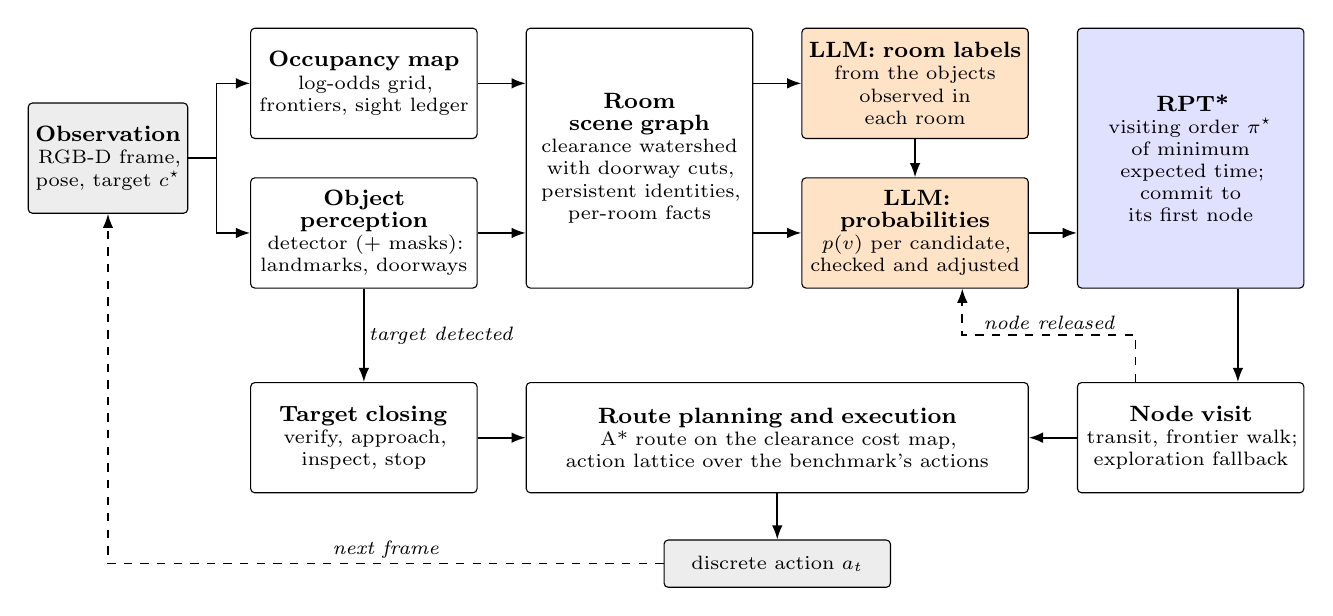
\begin{tikzpicture}[x=1mm, y=1mm, font=\scriptsize,
  box/.style={draw, rounded corners=1.5pt, align=center, inner sep=2.5pt,
              text width=27mm, minimum height=14mm, fill=white,
              execute at begin node={\hyphenpenalty=10000 \exhyphenpenalty=10000 }},
  tall/.style={box, minimum height=33mm},
  llm/.style={box, fill=orange!22},
  rpt/.style={tall, fill=blue!12},
  io/.style={box, text width=18.5mm, fill=black!7},
  arr/.style={-{Latex[length=1.8mm]}, semithick},
  back/.style={arr, dashed},
  note/.style={font=\scriptsize\itshape, inner sep=1.5pt}]
  % Perception and mapping, scene graph, language model, global planner
  \node[io]   (obs)   at (0,-9.5)    {\boxtitle{Observation}\\ RGB-D frame,\\ pose, target $\cstar$};
  \node[box]  (map)   at (32.5,0)    {\boxtitle{Occupancy map}\\ log-odds grid,\\ frontiers, sight ledger};
  \node[box]  (perc)  at (32.5,-19)  {\boxtitle{Object perception}\\ detector (+ masks):\\ landmarks, doorways};
  \node[tall] (graph) at (67.5,-9.5) {\boxtitle{Room scene graph}\\ clearance watershed\\ with doorway cuts,\\ persistent identities,\\ per-room facts};
  \node[llm]  (label) at (102.5,0)   {\boxtitle{LLM: room labels}\\ from the objects\\ observed in each room};
  \node[llm]  (prob)  at (102.5,-19) {\boxtitle{LLM: probabilities}\\ $p(v)$ per candidate,\\ checked and adjusted};
  \node[rpt]  (order) at (137.5,-9.5) {\boxtitle{RPT*}\\ visiting order $\pi^\star$\\ of minimum\\ expected time;\\ commit to its first node};
  % Execution
  \node[box]  (close) at (32.5,-45)  {\boxtitle{Target closing}\\ verify, approach,\\ inspect, stop};
  \node[box, text width=62mm] (nav) at (85,-45) {\boxtitle{Route planning and execution}\\ A* route on the clearance cost map,\\ action lattice over the benchmark's actions};
  \node[box]  (visit) at (137.5,-45) {\boxtitle{Node visit}\\ transit, frontier walk;\\ exploration fallback};
  \node[io, text width=27mm, minimum height=6mm] (act) at (85,-61) {discrete action $a_t$};
  % Data flow
  \draw[arr] (obs.east) -- ++(3.6,0) |- (map.west);
  \draw[arr] (obs.east) -- ++(3.6,0) |- (perc.west);
  \draw[arr] (map.east) -- (map.east -| graph.west);
  \draw[arr] (perc.east) -- (perc.east -| graph.west);
  \draw[arr] (label.west -| graph.east) -- (label.west);
  \draw[arr] (prob.west -| graph.east) -- (prob.west);
  \draw[arr] (label.south) -- (prob.north);
  \draw[arr] (prob.east) -- (prob.east -| order.west);
  \draw[arr] ([xshift=6mm]order.south) -- ([xshift=6mm]visit.north);
  \draw[arr] (perc.south) -- node[note, right] {target detected} (close.north);
  \draw[arr] (close.east) -- (nav.west);
  \draw[arr] (visit.west) -- (nav.east);
  \draw[arr] (nav.south) -- (act.north);
  % Feedback
  \draw[back] ([xshift=-7mm]visit.north) -- ++(0,6) -| node[note, pos=0.25, above] {node released} ([xshift=6mm]prob.south);
  \draw[back] (act.west) -| node[note, pos=0.25, above] {next frame} (obs.south);
\end{tikzpicture}
\caption{Overview of \ours. Every frame updates the occupancy map and the
landmarks, from which the room scene graph is rebuilt. At a loop point the
language model (orange) labels the rooms and estimates $p(v)$ for every
candidate room, RPT* (blue) orders the candidates, and the first is visited; a
detection of the target hands control to target closing. Every goal
is executed as discrete actions on the occupancy map. Dashed arrows are
feedback.}
\label{fig:overview}
\end{figure}

\begin{algorithm}[t!]
\caption{\ours: one episode; every iteration executes one action $a_t$.
Omitted: glances, the look-down before a narrow passage, the look-around that
revisits a finished room, the look at a target-landmark node, the pursuit of a
released target, the walk to a target landmark without a takeover, and starts
on a staircase
(\cref{sec:visits,sec:navigation,sec:nodes,sec:closing,sec:storey}).}
\label{alg:main}
\small
\begin{algorithmic}[1]
\Require target category $\cstar$; RGB-D frame $(I_t, D_t)$ and pose $x_t$ at every step $t$; action budget $T$
\Ensure \textbf{Found} (\code{STOP} at the target), or \textbf{Fail} when the budget is spent
\State \textbf{State:} occupancy map $M$; scene graph $G$; probabilities $p$; committed node $v$
\State $M \gets \emptyset$;\quad $G \gets \emptyset$;\quad $p \gets \emptyset$;\quad $v \gets \emptyset$
\For{$t = 1, \dots, T$}
    \State $B \gets \textsc{Detect}(I_t)$ \Comment{boxes of the vocabulary; masks for the target class}
    \If{\textsc{TargetCandidate}($B$)} \Comment{a candidate of $\cstar$ is active, or starts on $B$}
        \State $(M, G) \gets \textsc{UpdateSceneGraph}(M, G, B, D_t, x_t)$ \Comment{Alg.~\ref{alg:graph}, lines \ref{ln:graph-first}--\ref{ln:graph-last} only}
        \If{$\textsc{TargetClosing}(B, M, x_t) = \code{STOP}$} \Comment{Alg.~\ref{alg:closing}: one action $a_t$}
            \State \Return \textbf{Found}
        \EndIf
        \State \textbf{continue}
    \EndIf
    \State $(M, G) \gets \textsc{UpdateSceneGraph}(M, G, B, D_t, x_t)$ \Comment{Alg.~\ref{alg:graph}}
    \If{\textsc{WarmUp}()} \Comment{turns in place until ten were made: the first look-around}
        \State \textbf{continue}
    \EndIf
    \State $G \gets \textsc{ReadExits}(M, G)$ \Comment{exits of the rooms (Sec.~\ref{sec:rooms})}
    \If{$v \neq \emptyset$ and \textsc{Done}($v$)} \Comment{no significant frontier left, $60$ actions in $v$, or $v$ unreachable}
        \State $v \gets \emptyset$ \Comment{release}
    \EndIf
    \If{$v = \emptyset$} \Comment{loop point: choose the next node}
        \State $\Nodes \gets \textsc{CandidateNodes}(G)$ \Comment{rooms not finished, or re-offered; target landmarks (Sec.~\ref{sec:nodes})}
        \If{\textsc{QueryDue}()} \Comment{a node was searched, or the rooms or labels changed (Sec.~\ref{sec:oracle})}
            \State $G \gets \textsc{LabelRooms}(G)$ \Comment{LLM (Sec.~\ref{sec:labels})}
            \State $p \gets \textsc{RoomProbabilities}(\cstar, G, \Nodes)$ \Comment{Alg.~\ref{alg:prob}}
        \EndIf
        \State $c \gets \textsc{TravelCosts}(M, x_t, \Nodes)$ \Comment{Eq.~\eqref{eq:cost}}
        \State $\pi^\star \gets \textsc{RPT}^*(\Nodes, p, c)$;\quad $v \gets \pi^\star_1$ \Comment{Eq.~\eqref{eq:objective}; $v$ stays $\emptyset$ if no node is offered}
    \EndIf
    \If{$v = \emptyset$}
        \State $g \gets \textsc{ExplorationFallback}(M)$ \Comment{Sec.~\ref{sec:fallback}}
    \ElsIf{$v$ has not been reached}
        \State $g \gets \textsc{EntryPoint}(v)$ \Comment{committed transit (Sec.~\ref{sec:visits})}
    \Else
        \State $g \gets \textsc{BestFrontier}(v)$ \Comment{frontier walk: highest utility $U$, Eq.~\eqref{eq:viewgain}}
    \EndIf
    \State $a_t \gets \textsc{NextAction}(\textsc{A}^*(M, x_t, g))$ \Comment{A$^*$ route, then the action lattice (Sec.~\ref{sec:navigation})}
\EndFor
\State \Return \textbf{Fail}
\end{algorithmic}
\end{algorithm}

% ============================================================================
\section{Method}\label{sec:method}

\begin{algorithm}[t]
\caption{\textsc{UpdateSceneGraph}: the map and the room graph after a new
frame. During the walk to a committed room the rooms are rebuilt only every
fifth action, when the set of confirmed doorways changes, and when the walk
ends.}
\label{alg:graph}
\small
\begin{algorithmic}[1]
\Require occupancy map $M$; scene graph $G$; boxes $B$; depth $D_t$; pose $x_t$
\Ensure the updated $M$ and $G$
\State $M \gets \textsc{Integrate}(M, D_t, x_t)$ \Comment{log-odds grid; a refused step is written as an obstacle (Sec.~\ref{sec:mapping})}\label{ln:graph-first}
\State $M \gets \textsc{MaskStairs}(M, D_t, x_t)$ \Comment{staircases and drops are impassable (Sec.~\ref{sec:storey})}
\State \textsc{RecordSight}($M, x_t$) \Comment{sight ledger: the cells in view from $x_t$}
\ForAll{boxes $b \in B$}
    \State $G \gets \textsc{Fuse}(G, b, D_t, x_t)$ \Comment{3-D projection into a landmark of its class, or a doorway (Sec.~\ref{sec:perception})}
\EndFor\label{ln:graph-last}
\State \textsc{CreditAction}($G, x_t$) \Comment{one more action spent in the room of $x_t$}
\If{\textsc{RebuildDue}()} \Comment{every action, except during a committed walk}
    \State $F \gets \textsc{FreeCells}(M)$;\quad $d \gets \textsc{Clearance}(F)$ \Comment{Sec.~\ref{sec:rooms}}
    \State $C \gets \textsc{Cuts}(G, F)$ \Comment{confirmed doorways moved to chokes of $F$; thresholds on the trail and sight lines}
    \State $R \gets \textsc{Watershed}(-d, C)$ \Comment{seeded at the maxima of $d$, cut at $C$}
    \State $R \gets \textsc{Merge}(R, C)$ \Comment{saddle dynamics below $0.2\m$; never across a cut}
    \State $G \gets \textsc{MatchRooms}(G, R)$ \Comment{identities kept by anchor, overlap and containment}
    \ForAll{rooms $r \in G$}
        \State \textsc{UpdateFacts}($r$) \Comment{its landmarks, mapped floor and frontiers}
    \EndFor
\EndIf
\State \Return $M, G$
\end{algorithmic}
\end{algorithm}

\subsection{Occupancy mapping}\label{sec:mapping}
The map is a 2-D log-odds occupancy grid~\citep{elfes1989using} of
$80\m\times80\m$ at $0.1\m$ resolution, centred on the start position. Each
depth image is sub-sampled every $8$ pixels and back-projected with the pose
and the current camera pitch. Let $h$ be the height of the storey plane
(initially the start height). Points whose height lies in
$[h+0.15,\,h+0.93]\m$ are obstacle evidence: a cell that receives $n$ such
points in a frame is updated by
$L \leftarrow \mathrm{clip}(L + 0.85\,s,\,-4,\,4)$ with
$s=\mathrm{clip}(n/10,\,0.2,\,1)$, and every cell on the grid ray from the
camera to such a point by $L \leftarrow \mathrm{clip}(L-0.40,\,-4,\,4)$.
Points within $0.10\m$ of the plane are floor evidence and decrement their own
cell in the same way unless it is currently occupied. With
$P=1/(1+e^{-L})$, a cell is \emph{free} if $P\le0.45$, \emph{occupied} if
$P\ge0.65$ and \emph{unknown} otherwise or if never updated. The cells under
the body are free unless occupied.

\paragraph{Contact evidence.} The simulator refuses a forward step that would
collide. The agent detects this from its own pose (a \code{MOVE\_FORWARD} that
displaced it by less than $5\cm$) and sets the cell one step ahead to the
maximum log-odds, except for a scrape in a doorway (\cref{sec:navigation}). A
second refusal within $0.5\m$ of an earlier one writes a
bar one body wide across the heading that stays occupied for $120$ actions.
Conversely, cells on which the agent has stood are always treated as free by
the planner.

\paragraph{Frontiers and settled unknown.} A frontier cell is a free cell
4-adjacent to an unknown cell; frontier cells are grouped into 8-connected
clusters of at least four cells, and a cluster that wraps around a block of
unknown space is cut into one cluster per side. Not all unknown space is worth
exploring. A \emph{sight ledger} marks unknown cells as \emph{settled} when
(i) camera rays cast over the map ended at them within $2.5\m$ from at least
two distinct poses without the depth ever resolving them (a window, a railing,
a hole in the mesh), or (ii) they form an enclosed pocket of at most $3\sqm$
that is narrower than $0.6\m$ or that the agent has stood on. Settled cells
are ignored when frontiers, exits and view gains are computed; the planner
keeps using the real map.

\subsection{Object perception and landmarks}\label{sec:perception}
\paragraph{Detector interface.} The method consumes a generic detector: for
each frame, boxes with a class name from a closed vocabulary and a confidence.
The vocabulary consists of the prompts of the benchmark's goal categories plus
\emph{context} words that help to tell rooms apart (e.g.\ sink, oven,
refrigerator, bathtub), doorway words and a few distractors. Optionally a
segmenter returns a mask for each target-class box. The implementation
supports YOLO-World~\citep{cheng2024yolo} and box-prompted
SAM~\citep{kirillov2023segment} behind this interface; \emph{all our
experiments instead answer the interface from the simulator's semantic
annotations} (\cref{sec:experiments-oracle}).

\paragraph{From a box to a 3-D point.} A box with confidence at least $0.30$
is measured on the depth pixels it covers, or on its mask when one is given.
We take a robust depth for the region, keep the largest connected component of
pixels within a depth band around it, and require at least eight supporting
pixels (and, without a mask, that the component covers at least $35\%$ of the
valid pixels of the box's central region, so that a box spanning two surfaces
is rejected). The component is back-projected; its per-axis median is the
object's position and the $10$th percentile of its horizontal distances to
the agent is the \emph{near-surface range} used later for stopping. Without a
mask, a near surface that covers only part of a box in front of a second
surface spanning the whole box is treated as an occluder and removed before
the measurement. A projected object must lie between $0.3\m$ below and
$2.2\m$ above the storey plane and be supported by observed floor nearby.

\paragraph{Landmark map.} Projected objects are fused into landmarks. Two
observations of the \emph{same class} belong to one landmark when their
positions are within $0.35\m$ or their footprint discs overlap with an IoU of
at least $0.25$, and their heights differ by at most $0.35\m$; different
classes never merge. A landmark is \emph{confirmed} after two observations and
is retracted when it stood, unoccluded and in range, without a detection of
its class in as many views from distinct viewpoints as it has observations,
and in at least four.

\paragraph{Doorways.} Boxes of the doorway classes (accepted from confidence
$0.05$) are located from the depth of the door frame, not of what is seen
through it, and must pass geometric gates (apparent width $0.35$--$1.5\m$, top
at least $1.4\m$ and bottom at most $0.5\m$ above the floor). A doorway is
confirmed after three observations, at least one of them from a viewpoint
$0.2\m$ or $20\degree$ away from the first. Confirmed doorways constrain the
room partition and are recorded on rooms and their exits (\cref{sec:rooms});
a refused step in one counts as a scrape (\cref{sec:navigation}).

\subsection{Online room graph}\label{sec:rooms}
\paragraph{Partition.} Rooms are obtained from the current free mask alone,
without the footprints of staircases (\cref{sec:storey}).
Small holes are healed and the Euclidean clearance $d(\cdot)$ to the nearest
non-free cell is computed. Every local maximum of $d$ with $d\ge0.3\m$,
separated from other maxima by at least $1.0\m$, seeds a room, and a
watershed~\citep{vincent1991watersheds} of $-d$ grows the seeds until they
meet at the narrow places between them. Two kinds of cuts are forced before
the flood: (i) each confirmed doorway, moved to the narrowest \emph{choke} of
the medial axis within $0.9\m$ (a point of clearance between $0.25$ and
$0.8\m$ whose removal splits the skeleton into two substantial parts) and cut
across the passage there, or a disc of radius $0.75\m$ when no choke is found;
and (ii) \emph{thresholds}, points where the clearance dips to at most
$0.55\m$ and rises by at least $0.3\m$ on both sides within $1.5\m$, read off
the trail the agent has walked and off its lines of sight to the exits of
rooms (below). The watershed over-segments rooms that
have two wide areas; adjacent basins are therefore merged when the
\emph{dynamics} of their common saddle~\citep{grimaud1992new}, the smaller of
the two clearance peaks minus the clearance at the saddle, is below $0.2\m$,
never across a forced cut. Regions smaller than $50$ cells are dropped, except
floor glimpsed beyond a forced cut, which is a room from four cells.

\paragraph{Identity.} Rooms keep their identity when the partition is
recomputed. A new region inherits the identifier
of a previous room if it contains that room's birth anchor with sufficient
overlap, else by intersection-over-union (at least $0.15$), else by
containment (at least $0.6$); rooms that vanish are remembered and re-adopted
when they reappear, and identifiers are never reused.

\paragraph{Room facts.} For every room the graph keeps its area and elongation,
the confirmed landmarks credited to it (the room under the landmark, or the
nearest room floor within the landmark's footprint plus $0.6\m$, since
furniture stands on occupied cells), the number of reachable frontier clusters
inside it, the time the agent has spent in it and when it was last inside, and
its \emph{exits}: frontier clusters at the room's edge that lead to space not
seen yet, with whether a doorway was detected there, which objects were
glimpsed through them and how much unseen floor the camera could reach beyond
them. An exit is an attribute of its room, not a node of its own.

\subsection{Room labels from a language model}\label{sec:labels}
A room is named by a language model from what was observed in it. The prompt
(\cref{app:prompts-room}) lists the confirmed objects of the room with their
counts and its geometry (area, shape, number of doorways) and asks for one
label from a fixed set of twelve residential room types, five non-residential
ones and \code{unknown}, with a confidence. A room is classified as soon as it
holds one confirmed object; a room without objects is classified from its
geometry alone when it is at least $2\sqm$ and looks like a passage (elongation
of at least $2.5$, or two or more doorways). The label is revised when a new
kind of object appears in the room, when object counts change (at loop points)
and periodically (every $50$ actions); a changed verdict that is not backed by
a new kind of object is adopted only when the model repeats it. Each label
carries a \emph{strength}: it is \emph{strong} when it rests on at least two
kinds of object and the model's confidence is at least $0.65$, and
\emph{weak} otherwise. The strength is shown to the second LLM query (a weak
label is printed with a question mark); it does not exclude a room from the
search.

\subsection{Candidate nodes}\label{sec:nodes}
The candidates $\Nodes$ of \cref{eq:objective} are, in the single-storey
configuration, of two kinds.
\emph{Rooms}: every room of the current partition that is not \emph{finished}
(\cref{sec:visits}) and whose entry point has not repeatedly proved
unreachable.
\emph{Target landmarks}: a landmark of the target's own class that the map has
confirmed, or that was seen once with confidence of at least $0.5$, but that
did not trigger the closing behaviour (typically a far or weak detection). It
is offered at a fixed probability of $0.85$ without an LLM query and is visited
by walking to a point $1.5\m$ from it and looking at it.

\subsection{Per-room success probabilities from a language model}\label{sec:oracle}
\paragraph{Query.} At a loop point the model is shown the whole picture in one
prompt (\cref{app:prompts-oracle}) and is asked, for every candidate room, for
the probability \emph{that the target is in the part of that room the agent
has not seen yet}. The prompt gives the reason for this wording: a detector
examines every camera frame, so a target that has not been found lies in a
place that has not been seen. The number is used as
the $p(v)$ of \cref{eq:objective}, after the checks described below. The
prompt contains
(i) the name of the target category of the current episode, in every query;
(ii) a one-line summary of the home so far: the room types found and whether
each was entered or finished, the numbers of unidentified rooms and of exits
not looked into, whether unexplored frontier is reachable, and the actions
used; and
(iii) one line per room with four items and nothing else: its label (a weak
label is marked; a room without a label is printed as \code{unknown} followed
by the objects confirmed in it, with their counts, at most eight classes --- a
labelled room does not list its objects); the floor already mapped out of the
room's floor, in square metres and as a share (see below); the number of
frontier clusters left in the room; and the number of actions already spent
inside it, or \code{never} for a room that has not been entered.
\emph{No distance and no position enters the prompt}, neither a room's
neighbours nor which room the agent is standing in: weighing the probabilities
against travel, including walking through a searched room to reach another, is
the planner's task (\cref{sec:rpt}), and the prompt says so. The model
answers in
JSON with three short pieces of reasoning (where the target is normally found;
what the rooms found say about the building; how far the search has got), a
verdict on whether re-checking finished rooms is now worth more than what is
left unexplored (recorded, but not acted upon in the configuration reported
here), and, for every room, a justification of at most twelve words followed by
one integer percentage.

\paragraph{Mapped floor.} The two areas on a room's line are computed from the
agent's occupancy map and the current room partition, with the sight ledger of
\cref{sec:mapping}, and from nothing else.
The \emph{floor of a room} is the area of its free cells, i.e.\ floor on which
the agent can stand. Furniture standing in the room and enclosed pockets of
unknown space are not counted: floor that the agent cannot reach is not part of
the room for this purpose. The \emph{mapped} part is the area of those cells
that the camera has observed from at most $4\m$ with a free line of sight on
the map, at a camera pitch at which an object between $0.3$ and $1.0\m$ tall
standing on that cell would be in the image; it is thus the floor on which the
detector has had the opportunity to see the target. The prompt prints both
areas and their ratio in coarse steps, e.g.\ \code{mapped=6 of 12 m2 (50\%)},
because a share alone does not distinguish a small room from a large one. A
room whose floor continues beyond the map has frontier clusters,
and their number is on the same line. The record of observed cells is attached
to map cells and not to room identifiers, so these quantities remain correct
when the partition merges, splits or renumbers rooms.

\paragraph{What the prompt supplies, and what it leaves to the model.} The
system prompt (\cref{app:prompts-oracle}) tells the model to use its own
knowledge of standard homes and buildings (in which rooms furniture and
objects of each kind are normally found) and to derive every probability from
that. Beyond this it explains the fields of its input and fixes the reply
format. It also says, in three short
statements and without any number, what the search so far \emph{means}:
(a) the more of a room is mapped and the more actions have been spent
searching it, the less of it is left to hold the target;
(b) a room that was never entered has not been searched, and the more the
other rooms have been searched, the more likely the target is in it;
(c) a room's number concerns only whether the target is in that room, and a
searched room may still be walked through on the way to another.
These statements state a direction and no magnitude. The prompt contains no
knowledge of ours
about where objects are: it names no room for any object, gives no
probability, band, threshold or typical value, does not list the goal
categories of any benchmark, and contains no worked example. The target
category of the episode is the only object the model is asked about, and it
appears in the user prompt of every query.

The wording is specific to a language model, so the code keeps the prompt as
named \emph{versions}, each written for one model, and a test fails if a
version names an object or a room type, contains a number other than those of
the reply format, or lacks the instruction to use the model's own knowledge.
The version listed in \cref{app:prompts-oracle} was written for and tested on
Qwen2.5-3B-Instruct.

Three things outside this prompt are
hand-designed and are not the model's judgement: the vocabulary of room types
of the room labeller (\cref{sec:labels}), whose labels the model reads; the
rescaling of the model's numbers by exploration state (below); and the fixed
probability of a target-landmark node (\cref{sec:nodes}). Apart from the two
prompts no knowledge of where objects are found reaches the search: the code
contains no table that maps object categories to rooms.

\begin{algorithm}[t]
\caption{\textsc{RoomProbabilities}: the language model's reply, checked and
adjusted by exploration state.}
\label{alg:prob}
\small
\begin{algorithmic}[1]
\Require target $\cstar$; scene graph $G$; candidate rooms $\Nodes$; for a room $v$: $n_v$ actions spent inside it, $f_v$ significant frontiers
\Ensure $p_v$ for the rooms that are offered to RPT$^*$
\State $P \gets \textsc{Prompt}(\cstar, G, \Nodes)$ \Comment{the home in one line; per room: label, mapped floor, frontiers, $n_v$}
\State $r \gets \textsc{LLM}(P)$ \Comment{one percentage $r_v$ per room, in JSON; one retry}
\If{$r$ holds no usable number}
    \State \Return $\emptyset$ \Comment{exploration fallback; next query after $25, 50, \dots, 200$ actions}
\EndIf
\If{no $r_v$ exceeds $1$ and one lies in $(0, 1)$} \Comment{written as fractions}
    \State $r \gets 100\,r$
\EndIf
\ForAll{rooms $v \in \Nodes$}
    \State $p_v \gets \textsc{Clip}(r_v, 0, 100)$ \Comment{$r_v = 1$ for a room that is missing from the reply}
    \If{$v$ was never entered and $p_v < 1$}
        \State $p_v \gets 1$ \Comment{not looked at is not ruled out}
    \EndIf
    \State $p_v \gets \min\bigl(p_v / 100,\; 1 - 10^{-6}\bigr)$
    \If{$v$ was never entered}\label{ln:prob-adjust-first}
        \State $p_v \gets \min\bigl(1,\; \max(0.15,\; 1.5\,p_v)\bigr)$
    \ElsIf{$v$ was entered and left}
        \State $\phi \gets \max\bigl(0.05,\; 0.5 \cdot 2^{-n_v/20}\bigr)$ \Comment{halves with every $20$ actions spent inside}
        \If{$n_v \ge 20$ and $f_v \le 1$}
            \State $\phi \gets \min(\phi,\, 0.2)$
        \EndIf
        \State $p_v \gets \phi\, p_v$
    \EndIf\label{ln:prob-adjust-last}
\EndFor
\State \Return $\{\,p_v : p_v \ge 0.05\,\}$ \Comment{a target landmark enters at $p = 0.85$ without a query}
\end{algorithmic}
\end{algorithm}

\paragraph{From the reply to probabilities.} The model is not required to
write exactly what the planner needs. \Cref{alg:prob} gives the checks and the
adjustment that the code applies between the reply and RPT*. They use only the
reply and what the agent has done in each room, and contain no knowledge of
any object category or room type. Numbers written as text, with a percent
sign or under a substituted key are accepted, and identifiers that were not
offered are dropped. The numbers are \emph{not} normalised: several rooms may
each hold an instance, and \cref{eq:objective} treats them as independent;
they are kept below one because the heuristic of RPT* divides by $1-p$. An
omitted room was forgotten, not ruled out, and a zero for a room that was never
entered is read in the same way, since nobody has looked there: such a room is
always a candidate, at a probability that permits exploring it but does not
compete with a room the model is confident about. A zero for an entered room
is the model's verdict on what was observed there and is kept. The adjustment
by exploration state (lines \ref{ln:prob-adjust-first}--\ref{ln:prob-adjust-last} of
\cref{alg:prob}; the room the agent is standing in keeps its number) is hand-set, as a safeguard against a
model that ignores the effort already spent in a room. Since the prompt also
tells the model that this effort counts against a room (statement (a) above),
the same evidence can be counted twice for an entered room. Without a usable
reply the code does not substitute a uniform distribution: the exploration
fallback (\cref{sec:fallback}) acts until the query is repeated. Quantities
that change continuously (the action counts) are printed in coarse steps, and
a reply is reused without a call when the prompt is identical to the previous
one.

\paragraph{When the model is queried.} The oracle is queried at a loop
point: at the start and whenever a node has been searched and released.
While a node is in force, a change of a room's label or of the set of offered
rooms does not interrupt it; the query waits for the next loop point. While no
node is in force, a label change triggers a query at once and a change of the
set of offered rooms at most every $8$ actions (the partition renumbers rooms
frequently as the map grows). A node that was released because it could not be
reached does not trigger a query; the order is re-solved on the standing
numbers.

\subsection{Ordering by minimum expected time: RPT*}\label{sec:rpt}
\paragraph{Instance.} Each node is represented by its \emph{entry point}
(\cref{sec:visits}). The travel distance $d(u,v)$ between two entry points, and
from the agent to each, is the shortest path on the 8-connected graph of
passable grid cells, measured at the planner's preferred obstacle clearance
where that connects the two points and at its minimum clearance otherwise;
nodes that cannot be reached from the agent on the current map are withheld.
Distances are converted to time at one forward step ($0.25\m$) per action, and
the expected duration $\tau_v$ of searching $v$ is added to every leg entering
it:
\begin{equation}\label{eq:cost}
  c(u,v) \;=\; \frac{d(u,v)}{0.25\m} \;+\; \tau_v,
  \qquad
  \tau_v \;=\; \min\bigl(60,\; 4 + 4\,f_v\bigr)\ \text{actions},
\end{equation}
where $f_v$ is the number of significant frontiers in room $v$ ($\tau_v=4$ for
a target-landmark node). Two special cases: $\tau_v=20$ (half an approach plus
a full turn) for a room that was finished from outside and is offered again,
and $\tau_v=12$ when the room's frontier count is not available. Folding
$\tau_v$ into the entering legs preserves the triangle inequality of $d$, on
which the solver's pruning relies, and makes the planner discount the search time of a room by the
probability that the target was already found.

\paragraph{Solver.} We minimise \cref{eq:objective} with our own
implementation of RPT*~\citep{lyu2026rpt}, written from the paper's text (no
reference code was available to us): a best-first search over states that
consist of the current node, the set of visited nodes, the accumulated
expected cost and the survival probability $q$, with dominance pruning and an
admissible heuristic obtained from a relaxation that allows revisits. The
search is exact when it terminates within its time budget ($2$\,s); otherwise
it returns the best complete order found so far, or a nearest-neighbour order
if there is none, and marks the result as carrying no guarantee. If the
instance cannot be solved, which happens when legs measured at the two
clearances violate the triangle inequality on which the pruning relies, a
single node is drawn at random with probability proportional to $p$ (seeded
per episode). Because the
search is exponential in the number of nodes, at most $12$ nodes enter one
solve: the nearest node and the eleven most probable ones. The agent commits
to the first node of the returned order and the order is re-solved at the next
loop point. In the HM3D run of \cref{tab:main}\oldrev{} the solver returned a
provably optimal order in $99.3\%$ of its $8{,}657$ calls, each within
$11$\,ms and with at most $11$ nodes; the other $0.7\%$ were instances that
violated the triangle inequality.

\subsection{Visiting a room}\label{sec:visits}
\paragraph{Warm-up.} An episode starts with a rotation in place of ten
$30\degree$ turns, which is what the $79\degree$ camera needs to have seen
every bearing once. It gives the map its first rooms and the detector its first
objects, and it is recorded as a completed look-around of the start room.

\paragraph{Transit.} A room is entered at its \emph{entry point}: its most
valuable frontier (see below), or, if it has none left, its passable cell
nearest to the agent. The walk to the entry point is \emph{committed}: it ends
only by arrival, by a route that the planner refuses or on which the agent
makes no progress, by a timeout, or by a target detection. If the partition
renumbers the room on the way, the commitment follows the place. An entry point
that repeatedly cannot be reached is remembered by position and avoided for a
period that doubles with each failure.

\paragraph{Frontier walk.} Inside the room, the agent repeatedly walks to the
frontier of that room with the highest utility
\begin{equation}\label{eq:viewgain}
  U(g) \;=\; \frac{G(g)}
  {\bigl(\ell(g)+0.25\m\bigr)\,\bigl(1+|\Delta\theta(g)|/\pi\bigr)\,
   \bigl(1+0.05\,n(g)\bigr)},
\end{equation}
where $G(g)$ is the number of unknown, unsettled cells that a full turn of the
camera at $g$ would reveal (rays stop at occupied cells) plus the size of the
frontier cluster, $\ell(g)$ is the geodesic distance, $\Delta\theta(g)$ the
turn needed to face $g$, and $n(g)$ the number of actions the agent has already
spent within $1.5\m$ of $g$. Only \emph{significant} frontiers, those with at
least $1\sqm$ of revealable area, are walked to, kept as reasons to keep a
room open, or counted in $f_v$. The visit ends when no significant frontier is
left or after $60$ actions.

\paragraph{Finished rooms.} A ledger decides when a room needs no (further)
visit, from geometry alone:
(a) the agent completed a look-around inside it;
(b) a completed look-around elsewhere had at least $80\%$ of the room's cells in
unobstructed view within $4\m$, and the room has no significant frontier;
(c) the room has no significant frontier and the agent stood in it, at least
$0.5\m$ from its edge;
(d) it has no significant frontier and either is narrow (clearance of at most
$0.9\m$) and was walked through, or had at least $80\%$ of its cells in view
within $4\m$ from a single recorded pose;
(e) it has no significant frontier and is a fragment (under $3\sqm$ without a
doorway, or under $1\sqm$).
Finished rooms are neither shown to the oracle as nodes nor offered to the
planner (their types still appear in the summary line). Two exceptions bring a
finished room back: a room finished by a look-around that still has exits with
significant frontier is re-offered for what lies behind them, and rooms that
were finished from outside without ever being entered are re-offered once
every room is finished and no exit is left, and are then visited by a
look-around from a vantage point. A verdict is re-examined if the
room later grows by more than half.

\paragraph{Glances.} While walking, the agent may turn towards a confident
detection (at least $0.4$) that is cut by the left or right image border and
spans at least $30\%$ of the image height: always for the target class, and
for other classes only if that side still holds at least $2\sqm$ of unknown
floor. It turns at most
three times and then resumes its route.

\subsection{Exploration fallback}\label{sec:fallback}
When no node is in force (no room clears the probability threshold, every route
failed, or the language model is unavailable) the agent keeps moving by a fixed
ladder of rules, the first that yields a route being taken:
(1) the best reachable frontier on the storey by \cref{eq:viewgain}, excluding
frontiers that are probably the sensor shadow of an object, frontiers within
the camera's blind radius ($1.2\m$) and insignificant ones;
(2) such frontiers, insignificant ones included, with routes planned at the
body radius;
(3) the frontiers excluded in (1);
(4) frontiers that were given up earlier, and then any frontier that is
reachable when routes are planned at the body radius;
(5) a relocation to a far reachable cell for a new vantage point;
(6) a look down at the floor around the agent, turning a full circle, when the
agent is surrounded by unknown cells;
(7) a single probing step through the thinnest mapped barrier when the agent is
boxed in by occupied cells;
(8) a turn in place.
Rule (1) uses a short hand-written list of object classes that hide no floor
(e.g.\ clock, vase, book, television) and are therefore never treated as
casting a shadow. When rule (1) finds nothing, an episode that started on a
staircase may at that point use its one storey switch (\cref{sec:storey})
before the remaining rules are tried.

\subsection{Route planning and execution}\label{sec:navigation}
\paragraph{Routes.} Routes are computed with A*~\citep{hart1968formal} on the
8-connected grid. Unknown cells are not traversable. Occupied cells are
inflated by a preferred clearance of $0.30\m$; the planner relaxes this in
$5\cm$ steps down to $0.25\m$ when no route exists or when the route at the
preferred clearance is more than $1.5$ times longer than the relaxed one. The
cell cost adds two soft terms to the unit cost: a clearance term that decays
with distance from obstacles, and a centreline term
$4\,(1-d/0.6\m)$ for cells with clearance $d<0.6\m$, which makes a route cross
a doorway through its middle. A turn penalty discourages staircase-shaped
paths, and the result is simplified by removing near-collinear points and its
corners are rounded. A route is kept as long as its goal has not moved and it
remains collision-free on the updated map.

\paragraph{From route to actions.} The benchmark's motion is discrete:
$0.25\m$ steps and $30\degree$ turns, with any contact refusing the step.
Following a 2-D route with a waypoint controller cuts corners into door jambs.
Instead, every route is refined by a search in the spirit of
Hybrid~A*~\citep{dolgov2010path} over states (position, heading) whose only
transitions are the benchmark's own forward step and turns. A turn costs one
unit; a forward step costs the mean cost of the cells it crosses on the route
planner's cost map (one on open floor) and additionally pays for its lateral
offset from the 2-D route. The search is confined to a $0.4\m$ corridor around
the route and collision-checked against the clearance field. The resulting
action sequence
is executed open loop while the pose matches the plan (to $2\cm$ and
$1\degree$); a small displacement re-anchors the plan, anything else triggers
re-planning from the true pose. A refused step is also remembered as a
\emph{pose} from which stepping forward is excluded for $120$ actions. If the
lattice search finds no plan, a simple waypoint-following rule is used.

\paragraph{Narrow passages.} Two rules address doorways. A refused step in a
confirmed doorway, taken within $40\degree$ of the doorway's axis, is treated
as a scrape and is \emph{not} written into the map; once three scrapes at the
same place have been excused within $40$ actions, further refusals there are
written. And when a route is about to enter a passage
narrower than $0.9\m$, the camera is pitched down by $30\degree$ once so that
the floor of the passage, which a level camera does not see closer than about
$1.4\m$, is mapped before the agent enters.

\subsection{Target closing}\label{sec:closing}
A detection of the target category suspends the search and hands control to a
state machine (\cref{alg:closing}) that either ends the episode with
\code{STOP} or releases the candidate and returns to the search.

\begin{algorithm}[t]
\caption{\textsc{TargetClosing}: one action while a candidate of the target
class is active. \textbf{Release} gives the candidate up and returns control
to the search. The special cases of \cref{sec:closing} are omitted.}
\label{alg:closing}
\small
\begin{algorithmic}[1]
\Require boxes $B$; occupancy map $M$; pose $x_t$; stop distance $d_{\mathrm{stop}}$
\Ensure an action, \code{STOP}, or \textbf{Release}
\State \textbf{State:} remembered position $m$ of the candidate; flags \emph{locked}, \emph{inspecting}, \emph{stopping} (false at the start)
\State $\rho \gets$ near-surface range of a fresh box of the candidate in $B$; $\infty$ without one
\If{\emph{stopping}} \Comment{the stop was decided on an earlier frame}
    \State \Return \textsc{StopWalk}($m, d_{\mathrm{stop}}$) \Comment{\code{STOP} within $d_{\mathrm{stop}}$ or at a bound of the walk; else a step towards $m$}
\EndIf
\State \emph{locked} $\gets$ \emph{locked} or \textsc{SameObject}($B$) \Comment{two consecutive boxes project onto the same object}
\If{\textsc{BudgetSpent}()} \Comment{$160$ actions; or not locked after $12$, or after $6$ in a row with the box out of view}
    \State \Return \textbf{Release}
\EndIf
\If{not \emph{locked}} \Comment{verify}
    \State \Return \textsc{FaceAndStep}($B$) \Comment{face the box, step towards it; back off if it was first seen within $1.3\m$}
\EndIf
\State \emph{inspecting} $\gets$ \emph{inspecting}, or $\rho \le 1.05\m$, or $\rho = \infty$ and $\lVert x_t - m \rVert \le 1\m$
\If{not \emph{inspecting}} \Comment{approach}
    \State $s \gets \textsc{Standoff}(m, M)$ \Comment{ring around $m$, front first: standing floor with an A$^*$ route}
    \If{$s = \emptyset$}
        \State \Return \textsc{NoRoute}($m, M$) \Comment{nearest standing floor; look down and around; detour; else \textbf{Release}, keeping $m$}
    \EndIf
    \If{$x_t$ is not at $s$, or $\rho$ is finite and beyond $1.05\m$ by more than one step}
        \State \Return $\textsc{NextAction}(\textsc{A}^*(M, x_t, s))$ \Comment{\textbf{Release} if no progress was made in $20$ actions}
    \EndIf
    \State \emph{inspecting} $\gets$ true
\EndIf
\If{$\rho \le 1.05\m$ and \textsc{Aligned}(), or \textsc{MemoryCase}()} \Comment{inspect; aligned: centred, or tracked over the approach}
    \State \emph{stopping} $\gets$ true;\quad \Return \textsc{StopWalk}($m, d_{\mathrm{stop}}$) \Comment{the stop is decided}
\ElsIf{$\rho$ is beyond $1.05\m$ by at most one step, the box is faced, and fewer than three steps were made}
    \State \Return \textsc{StepForward}()
\ElsIf{$24$ actions were spent inspecting, or every view was tried without a box}
    \State \Return \textbf{Release} \Comment{the place is remembered}
\EndIf
\State \Return \textsc{NextView}() \Comment{centre the box, or turn and tilt to the next view}
\end{algorithmic}
\end{algorithm}

\paragraph{Start and lock.} A takeover starts on a box of the target class
with confidence of at least $0.5$ that has a valid 3-D projection, is not a
narrow fragment at the image border (a box cut only at the bottom by the floor
is accepted),
and is not near a place where a candidate was rejected before (a confidence of
at least $0.8$ overrides most rejection memories). The candidate becomes a
\emph{lock} after two consecutive frames whose projections fall on the same
object; while a candidate is active, boxes down to confidence $0.3$ count as
re-sightings if they project onto it. If the candidate is in view during the
verification but its box has no usable depth, the agent faces it and steps
towards it to obtain one; up to $24$ such steps are not counted against the
$12$ actions of the verification.
Three special cases
are handled: a first box that is too far for usable depth starts a bounded
walk along its bearing until a candidate can be placed; a candidate first seen closer than
$1.3\m$ is re-examined from a few steps back unless it was already seen in
recent frames or is very confident; and a candidate whose measured height is
outside a hand-set, per-class band (\cref{sec:handdesigned}) is not refused
but doubted: its confidence counts at $0.7$ of its value towards the start
threshold, and it needs four frames from two viewpoints at least $0.3\m$
apart.

\paragraph{Memory.} The position of a locked target is a precision-weighted
fusion of its associated observations, with a measurement noise that grows
with range. A re-sighting is associated to the lock if it falls within a
cylinder around the line of sight to the remembered position.

\paragraph{Approach.} The agent walks to a \emph{standoff} point on a ring
around the remembered position whose radius is chosen so that arriving puts
the agent within $1\m$ of the target (about $0.65\m$ with our tolerances).
Candidate points are tried in a fixed order: first on the side from which the
target was seen, then beside and behind it; for each, the default planner and,
if it finds no route, a planner at a smaller clearance (below).
Wider rings are tried when no point of the first ring is reachable.

\paragraph{Standing points.} Every point at which the closing asks the agent
to stand (a standoff point, the spot of the back-off manoeuvre, and the
closest floor used when no standoff has a route) is taken from the agent's own
occupancy map. A cell is \emph{standing floor} if
(i)~it has been observed free;
(ii)~every cell whose centre lies within the body radius ($0.18\m$) of its
centre has been observed free as well, so that neither an obstacle nor
unobserved space lies under the agent's body; and
(iii)~it is connected to the agent's position through cells that satisfy (i)
and (ii).
There is one such floor, and two planners are asked for a route on it, the
second only when the first finds none: the default planner, which keeps
$0.25\m$ of clearance from every observed obstacle, and a planner that keeps
the body radius ($0.18\m$). On the $0.1\m$ grid the centre of the nearest
obstacle cell is then at least $0.28\m$ and $0.20\m$ from the agent's cell;
no route is planned at a smaller clearance. Unobserved cells
do not count towards the planner's clearance: beyond the body's own disc
nothing has to have been observed. A
candidate point is moved to the nearest standing-floor cell within $0.5\m$
($0.15\m$ for the back-off spot) that is not separated from it by an observed
obstacle, and is discarded if there is none; the route is then planned to
exactly that cell. An unobserved cell is therefore never stood on, never
counted as clearance and never crossed, and a standoff is given up as soon as
the map no longer shows it as standing floor.

A level camera does not see the floor closer than about $1.4\m$, so the floor
in front of a target seen through a doorway is often not yet on the map, while
the floor of the room behind the target's wall is. Two rules keep the agent
from walking around that wall. A standoff whose walk over standing floor is
longer than $1.5$ times the range to the target plus $1\m$ is set aside. And
as long as a point in front of the target lies on unobserved floor, so is a
standoff beside or behind the target, or one from which the map shows an
obstacle before the target. When no standoff is left, the fallbacks of
\cref{alg:closing} apply: the walk to the nearest standing floor only if it
brings the agent closer, and the look down and around only once, if much of
the floor around the agent is unobserved. Within $1.5\m$ of the target the camera pitch is servoed to keep the
box inside the image.

\paragraph{Stop.} In the inspection the agent \emph{decides} to stop on a
fresh box of the target whose near-surface range is at most $1.05\m$ and
which is \emph{aligned}: centred in the image, or of a target that was tracked
over the approach. Without such a box the decision is taken only in narrow
\emph{memory cases}: when the inspection's actions are spent and a box within
range was seen during it; when the map shows a free line of sight to the
remembered position and either the target was tracked over the approach and
detected within its last $15$ actions, or the actions are spent and the
furniture that carries it is still detected there; or when no closer standing
point is reachable, a fresh box lies within one step of the limit and the
inspection's steps are spent or refused. An inspection in which a fresh box
reads more than one step beyond the limit returns to the approach, at most
three times.

How close the agent must then \emph{stand} is defined by the benchmark's
success region (\cref{sec:experiments-benchmarks}), so the closing takes a
\emph{stop criterion} as a parameter: a distance $d_{\mathrm{stop}}$ and a
measure. Let
$r$ be the horizontal distance from the agent to the nearest measured point
of the target, and $h$ the height of the lowest measured point of the target
above the floor under the agent, taken as zero below $0.3\m$ (an object that
stands on the floor). Under the \emph{planar} measure the range is $r$; under
the \emph{Euclidean} measure it is $\sqrt{r^2+h^2}$. Both are distances from
the agent's position on the floor to the extent of the object as the agent
has measured it. Apart from the $0.3\m$ threshold, which changes a range of
$0.9\m$ by less than $0.05\m$, neither is smaller than the true distance to
the object's bounding box, so that an agent within the criterion by its own
measurement is within it of the object. If the range exceeds $d_{\mathrm{stop}}$ when the stop
is decided, the agent walks straight towards the remembered position and
issues \code{STOP} as soon as the range is within $d_{\mathrm{stop}}$. The
range is that of the deciding frame, carried forward by the agent's own
displacement; no detection is consulted during the walk, because close to a
raised target the box leaves the image. The walk also ends, with \code{STOP},
when a step is refused, after four steps or seven actions, when a further step
would bring the agent within $0.3\m$ of the remembered position or within its
body radius of the target's measured near edge, or on the last action of
the episode's budget; a target whose underside is higher than
$d_{\mathrm{stop}}$ is thus approached as closely as the body allows. Without a stop criterion ($d_{\mathrm{stop}}=0$, the method's
default) \code{STOP} is issued on the deciding frame. The agent is given no
goal position and no view point (\cref{sec:experiments-privileges}).

\paragraph{Release.} A release (\cref{alg:closing}) remembers the
place (radius $1\m$, doubled after a failed inspection) so that the same
detection does not restart the takeover from the same spot; a release for want
of a route, at the action bound, or from a standoff that the map shows to have
had no line of sight to the target remembers the agent's own position instead.
A lock that
was released only for want of a route is kept and pursued again, within a
bounded number of actions, once the map offers a route. A box of the target
class on which no takeover starts, for instance a close view from the spot of
an earlier release, still marks its landmark: while that landmark was seen
within the last $8$ actions the search walks towards it, and it issues
\code{STOP} within $0.75\m$ of it once the landmark has been observed in three
frames from viewpoints $0.2\m$ or $20\degree$ apart. A takeover that starts on
the way has precedence.

\subsection{Single-storey confinement}\label{sec:storey}
The search does not change storeys. The agent tracks the height
of the floor it stands on from its pose. Staircases are recognised from the
agent's own depth as support surfaces that rise or fall in steps, and their
footprint is written as impassable into the planning map; so is every cell
whose observed floor lies more than $0.30\m$ below the storey plane, or that a
depth ray crossed more than $0.45\m$ below it. Single steps and raised or
sunken parts of the same storey remain free: floor that the agent's depth
shows to be connected to the storey by risers it can climb (at most
$0.24\m$, with head room for the body) and that lies within $0.45\m$ of the
storey plane. That bound is the agent's own. It is the height difference at
which the agent's storey tracking reads the agent as having left the storey,
and it is well below the smallest height difference that the tracking accepts
between two storeys ($1.5\m$); floor further from the plane is not offered
because the same tracking would walk the agent back from it. A goal is refused
while the level the agent stands on is more than $0.5\m$ from the start
height; a split level less than $1.5\m$ from it, on which the agent has
settled for $30$ actions, is adopted as part of the start storey.
No simulator geometry is used for any of this, and none of these bounds is
taken from how a benchmark places or scores its goals (two checks against
evaluation data are disclosed in \cref{sec:experiments-privileges}).

\paragraph{Starts on a staircase.} Some episodes start on a stair tread or
landing, where no floor is level with the agent. In that case the first storey
the agent settles on becomes its storey: it walks the flight it sees to the
nearer end. A walk along a flight that fails is retraced, and if the retreat
does not end on level floor within $80$ actions the agent ends the episode
with \code{STOP}. The implementation additionally allows such an episode \emph{one}
switch to the storey at the other end of the same flight, and never back: once
the first storey has been searched out, or after $220$ actions on it, provided
that no target is known there and at least $120$ actions remain. Until the
agent has walked level on a
storey, floor within $0.8\m$ of its start height counts as connected in the
sense above (a hand-set value between the $0.45\m$ bound and the $1.5\m$
separation of two storeys). In all other episodes the agent stays on
its start storey. No staircase is a candidate node of \cref{eq:objective}.
Offering one requires knowing which storey a flight leads to, and the agent's
own stair detection measures the steps of a flight, not where it ends;
multi-storey search is left to future work.

\subsection{What is hand-designed}\label{sec:handdesigned}
The method is training-free, but it is not free of design choices, and several
of them encode knowledge about homes or about the benchmark. For transparency
we list them in one place.
\begin{itemize}[leftmargin=*,itemsep=1pt,topsep=2pt]
  \item \textbf{The two prompts} (\cref{app:prompts}). The oracle's system
        prompt describes its input and output and contains no statement about
        where objects are, no numeric band and no example
        (\cref{sec:oracle}); the room labeller's prompt fixes the set of room
        types and gives hand-written hints for naming a room from its objects
        (\cref{sec:labels}).
  \item \textbf{The rescaling of the model's probabilities} by exploration
        state (\cref{sec:oracle}) and the fixed probability of a
        target-landmark node (\cref{sec:nodes}).
  \item \textbf{Three small tables about object classes}, none of which says
        where a target is: per-class height bands used to doubt a candidate
        (bed, toilet, sofa, chair, potted plant, television;
        \cref{sec:closing}); a list of furniture classes that can carry other
        objects, used so that a detection of the supporting furniture counts
        for a locked target and not against it; and the list of classes that
        hide no floor
        (\cref{sec:fallback}).
  \item \textbf{Alias tables.} Synonymous class names
        are folded by small alias tables (e.g.\ couch and sofa; tv, monitor
        and television; armchair and chair), and synonymous room names in the
        model's replies likewise (e.g.\ corridor and hallway, study and
        office).
  \item \textbf{The detector vocabulary}: the context words given to the
        detector besides the goal categories.
  \item \textbf{The stop criterion}
        (\cref{sec:closing,sec:experiments-benchmarks}): $0.9\m$, measured
        horizontally on HM3D and in three dimensions from the floor on MP3D.
        These values state where each benchmark's published success region
        lies: the $1\m$ is the dataset generator's, and how it is measured was
        established on the validation goals
        (\cref{sec:experiments-privileges}). The margin of $0.1\m$ and the
        bounds of the walk are set by hand, the bounds after inspecting
        validation episodes.
  \item \textbf{All numeric thresholds} (\cref{app:hyperparams}). They were set
        by hand during development on the same validation episodes that we
        report (\cref{sec:experiments-privileges}).
\end{itemize}

% ============================================================================
\section{Experimental Setup}\label{sec:experiments}

\subsection{Benchmarks and protocol}\label{sec:experiments-benchmarks}
We evaluate on the validation splits of two Habitat ObjectNav benchmarks, each
in full:
\begin{itemize}[leftmargin=*,itemsep=1pt,topsep=2pt]
  \item \textbf{HM3D}~\citep{ramakrishnan2021habitat,yadav2023habitat}: the
        ObjectNav v1 episodes, $2{,}000$ episodes in $20$ scenes, with six
        goal categories (chair, bed, plant, toilet, tv\_monitor, sofa).
  \item \textbf{Matterport3D (MP3D)}~\citep{chang2017matterport3d}: the
        ObjectNav v1 episodes, $2{,}195$ episodes in $11$ scenes, with $21$
        goal categories (listed in \cref{tab:mp3d-cat}).
\end{itemize}
Both use the agent and the rules of \cref{sec:task}. We run
habitat-sim~0.2.4~\citep{savva2019habitat,szot2021habitat} through our own
adapter, which reproduces the episode and measurement rules of habitat-lab's
ObjectNav task, with a navigation mesh recomputed for the agent's dimensions
(radius $0.18\m$, height $0.88\m$). Every episode of
both splits is run; none is skipped, filtered or restarted. Both runs use a
single seed. As a check of the evaluation code, the start-to-goal geodesic
distances computed by our adapter agree with those published with the episodes
to within $1$\,mm on all MP3D episodes and on $1{,}992$ of the $2{,}000$ HM3D
episodes (largest difference $0.09\m$).

\paragraph{The success region, and the stop criterion derived from it.}
Success is defined through the view points that are published with each
episode, so the place where an agent must stand is determined by how the
authors of a dataset generated them. In the dataset generator of habitat-lab,
candidate positions are laid out on a horizontal grid around the axis-aligned
bounding box of a goal object, with a spacing of half the agent's radius
($0.09\m$) and out to $1\m$ from the box; a candidate becomes a view point if
it is navigable and the object is visible from it. We measured the view
points of every validation goal against the bounding box of the object in
the scene annotation and found that the two datasets differ in how this
$1\m$ is measured.
On HM3D ($432$ goals in $20$ scenes, $111{,}406$ view points) the farthest
view point of a goal lies $1.00\m$ from the box \emph{in the horizontal
plane}, whatever the height of the object, and no view point lies further
than $1.01\m$.
On MP3D ($1{,}316$ goals in $11$ scenes, $291{,}810$ view points) the
horizontal reach decreases with the height of the object's underside: its
median over goals is $1.00\m$ for objects on the floor, $0.89\m$ for an
underside between $0.3$ and $0.6\m$, $0.74\m$ between $0.6$ and $0.9\m$, and
$0.57\m$ between $0.9$ and $1.0\m$, while the three-dimensional distance from
the view point on the floor to the box stays at $1.00\m$; no goal has its
underside $1\m$ or more above the floor.\footnote{About $5\%$ of the MP3D view
points lie further than $1\m$ from the box in the plane, where the generator
moved them onto the navigation mesh. The generator code that is publicly
available measures in the plane; the MP3D episodes do not follow it.}
The success region of an HM3D goal is thus the floor within $1\m$ of the
object in the plane, and that of an MP3D goal the floor within $1\m$ of the
object in three dimensions. We give the method the corresponding stop criterion
(\cref{sec:closing}): the planar measure on HM3D and the Euclidean measure on
MP3D, with $d_{\mathrm{stop}}=0.9\m$ on both. The margin of $0.1\m$ is chosen
so that a stop at $d_{\mathrm{stop}}$ is within the success distance of a grid
candidate inside the region whatever the offset of the grid (no position is
further than $0.064\m$ from a candidate), and leaves the remainder for the
error of the agent's own range. This is the only information about the
benchmark's scoring that the method receives
(\cref{sec:experiments-privileges}).

According to their released code, published zero-shot methods stop on a
horizontal range to the mapped points of the target on both datasets:
VLFM~\citep{yokoyama2024vlfm} below $0.9\m$,
ASCENT~\citep{gong2025stairway} at $0.6\m$ after stepping towards the target
from $1\m$, and ApexNav~\citep{zhang2025apexnav} within $0.2\m$ of the free
cell nearest a point $0.5\m$ from the object, with the success distance set to
$0.2\m$ in its evaluation configuration. None measures in three dimensions.

\subsection{Metrics}\label{sec:experiments-metrics}
For episode $i$ let $S_i\in\{0,1\}$ denote success, $l_i$ the geodesic distance
from the start to the nearest goal view point, $p_i$ the length of the path the
agent travelled, and $d_i$ the geodesic distance to the nearest goal view point
when the episode ends. We report the success rate
$\mathrm{SR}=\tfrac1N\sum_i S_i$; success weighted by path
length~\citep{anderson2018evaluation},
$\mathrm{SPL}=\tfrac1N\sum_i S_i\,l_i/\max(p_i,l_i)$; its soft variant
$\mathrm{SoftSPL}=\tfrac1N\sum_i \max(0,\,1-d_i/l_i)\,l_i/\max(p_i,l_i)$; and
the mean final distance to the goal, $\mathrm{DTG}=\tfrac1N\sum_i d_i$.
Intervals are at the $95\%$ level: Wilson score
intervals~\citep{wilson1927probable} for SR and percentile bootstrap
intervals~\citep{efron1979bootstrap} over episodes for SPL.

\subsection{Language model}\label{sec:experiments-llm}
Both queries of the method, the room labels of \cref{sec:labels} and the
per-room probabilities of \cref{sec:oracle}, are answered by the same
off-the-shelf model, served locally by Ollama in its 4-bit quantisation. The
model receives text only; it never sees an image. The reported runs used
Qwen2.5-14B-Instruct~\citep{qwen25} (\code{qwen2.5:14b-instruct}); the
benchmark launcher now defaults to the smaller Qwen2.5-3B-Instruct, for which
the prompt of \cref{app:prompts-oracle} was written. We use
temperature $0$ with a fixed seed, the server's JSON-constrained output mode, a
context window of $8{,}192$ tokens, and reply limits of $768$ tokens for a room
label and $1{,}536$ tokens for the probabilities. The model is used as
released: there is no fine-tuning, no retrieval and no in-context example
(the prompt of the reported runs contained one, \cref{sec:results-checks}).

\subsection{Perception: simulator annotations in place of a detector}
\label{sec:experiments-oracle}
All our experiments answer the detector and segmenter interfaces of
\cref{sec:perception} from the simulator's semantic annotations (the
HM3D-Semantics annotations~\citep{yadav2023habitat} and the Matterport3D object
annotations~\citep{chang2017matterport3d}) instead of from learned models. The
results are therefore an \emph{upper bound with respect to perception}: they
measure mapping, reasoning, planning and execution given ideal detections.
Precisely:
\begin{itemize}[leftmargin=*,itemsep=2pt,topsep=2pt]
  \item \textbf{Boxes.} For every frame the simulator renders an instance-id
        image. Every annotated instance that is visible in the frame, covers at
        least $64$ pixels and maps to a word of the detector vocabulary is
        reported once, with the tight box of its visible pixels and confidence
        $1.0$. The confidence thresholds of
        \cref{sec:perception,sec:nodes,sec:visits,sec:closing} therefore never
        bind in these experiments.
  \item \textbf{Masks.} The mask of a target-class box is the set of that
        instance's own pixels.
  \item \textbf{Which instances are the target.} For a goal category that the
        scene's episodes ask for, the instances reported under that category
        are \emph{exactly the instances that the episode dataset lists as its
        goals}. An instance whose annotation names the same category but which
        the dataset does not list as a goal is not reported at all. The oracle
        therefore never produces a target detection that the benchmark would
        not accept, which no detector that recognises a category from
        appearance can guarantee. This is stronger than category-level
        ground-truth semantics and must be kept in mind when reading the
        numbers. (In a scene without episodes for a category, its instances
        are reported by annotation name.)
  \item \textbf{Other classes.} Context and doorway classes are assigned from
        the annotation names by a fixed table (for MP3D also from the
        \emph{mpcat40} class, for doors, stairs, mirrors and curtains).
        Instances whose name has no entry are not reported.
  \item \textbf{Mis-registered annotations.} In some scans the semantic mesh
        is not registered to the rendered mesh everywhere, so that the sensor
        paints an object onto a surface metres away from it. A pixel with a
        depth reading is therefore kept only if that reading places it inside
        the
        instance's annotated 3-D bounding box inflated by $0.25\m$, and an
        instance with fewer than half of its measurable pixels inside that box
        is not reported. Twelve of the MP3D failures are nevertheless
        attributed to such phantom detections (\cref{sec:results-failures}).
\end{itemize}
Everything downstream of the two interfaces, from the projection of boxes to
the landmark map, the doorway finder and the closing behaviour, runs
unchanged.

\subsection{Privileged inputs}\label{sec:experiments-privileges}
For clarity we list everything the agent receives that a physical robot with
an RGB-D camera would not have.
\begin{enumerate}[leftmargin=*,itemsep=2pt,topsep=2pt]
  \item \textbf{Pose.} The exact pose of the simulator (position, heading and
        camera pitch) at every step, as is standard in this benchmark.
  \item \textbf{Depth.} Noise-free depth, with the range limit and the
        hole-filling rule of \cref{sec:task}.
  \item \textbf{Semantic perception.} The oracle of
        \cref{sec:experiments-oracle}, including its use of the benchmark's
        goal list to decide which instances are the target.
\end{enumerate}
The agent does \emph{not} receive goal positions or view points, distances to
the goal, a success signal, a collision flag (it infers a refused step from
its own pose), or any scene geometry: it has no access to the simulator's
navigation mesh or path finder, and it is given no storey or staircase
annotations. Of the benchmark's definition of success it is given the stop
criterion of \cref{sec:experiments-benchmarks}: one distance and one measure
per dataset, the same for every episode and every object. The navigation mesh is used only outside the agent: by the
simulator to move the agent, by the benchmark to place it and to measure the
distances that are scored, and by our analysis of the results by storey
(\cref{sec:results}). The episode description handed to the agent carries
identifiers, the category name, the camera, the action set and the step
budget, and nothing else; the evaluation harness refuses an episode that
carries navigation-mesh, storey or staircase data, and a test fails if any
module of the method can reach them.
This holds for the method as described; the earlier revisions behind the
reported runs still projected the standing points of target closing onto the
navigation mesh (\cref{sec:results-checks}).

\paragraph{Development on the evaluation data.} The method has no trained
parameters, but its rules and thresholds were developed by inspecting its
behaviour on validation episodes of these two benchmarks (and of Gibson), the
same splits that we report. We have no held-out measurement. The numbers below
are development-set numbers and are likely to be optimistic. Four further
uses of evaluation data or scene annotations during development are disclosed
here; the agent receives none of them. The rule for mapped floor
(\cref{sec:oracle}) was developed on recorded HM3D validation episodes, and
its areas were checked once against the room outlines annotated in the
Matterport3D scenes. One bound of the storey confinement was checked against
the simulator's navigation mesh: that floor further than $0.45\m$ from the
storey plane is not offered to the agent (\cref{sec:storey}). On the HM3D
validation episodes whose goal is on the start storey and that start on level
floor, no shortest path computed on the navigation mesh leaves that band. The
bound itself is the agent's own (\cref{sec:storey}), and the check did not
change the value. The $0.8\m$ band of a start on a staircase
(\cref{sec:storey}) was also looked at against validation goals. The stop
criterion of each benchmark
(\cref{sec:experiments-benchmarks}) was established by measuring the published
view points of the validation goals against the bounding boxes of the scene
annotations.

\subsection{Compute}\label{sec:experiments-compute}
Both runs used one workstation with a single 24\,GB GPU (NVIDIA RTX~4090),
which hosted the language model and the simulator's renderers, 24 CPU cores and
64\,GB of memory, with eight (MP3D) or nine (HM3D) episodes running in
parallel. The HM3D run took $24.0$ hours of wall-clock time and the MP3D run
$27.2$ hours; an episode took $372$\,s and $343$\,s on average. The language
model is the bottleneck. An episode issued on average $5.5$ (HM3D) and $4.9$
(MP3D) probability queries and $27.6$ and $24.9$ room-label queries; in the
MP3D run a probability query had on average $3{,}306$ prompt tokens and $162$
reply tokens, a room-label query $453$ and $43$. Every answer of the model was
recorded, so that any episode can be replayed exactly.

% ============================================================================
\section{Results}\label{sec:results}

All numbers in this section are subject to three caveats: oracle semantic
perception (\cref{sec:experiments-oracle}), development on the evaluated
episodes (\cref{sec:experiments-privileges}), and earlier revisions of the
code (\cref{sec:results-checks}).

\subsection{Main results}\label{sec:results-main}

\begin{table}[t]
\centering
\caption{Full validation splits under oracle semantic perception with the
search confined to the start storey. SR, SPL and SoftSPL in percent, with
$95\%$ intervals in brackets where they were computed; DTG in metres; Steps is
the mean number of actions per episode. \oldrev{}All rows are from two runs of
earlier revisions of the code, a different one for each benchmark
(\cref{sec:results-checks}). The
storey of the goal is determined after the fact from the simulator's
navigation mesh and is unknown to the agent; the two benchmarks use different
rules for it (see text).}
\label{tab:main}
\small
\setlength{\tabcolsep}{4.5pt}
\begin{tabular}{@{}llrllrrr@{}}
\toprule
Benchmark & Episodes & $N$ & SR & SPL & SoftSPL & DTG & Steps \\
\midrule
HM3D val & all                    & 2{,}000 & 71.0\oldrev{} [68.9, 72.9] & 39.8\oldrev{} [38.4, 41.2] & 41.0 & 3.15 & 248 \\
         & goal on start storey   & 1{,}652 & 83.5\oldrev{} [81.7, 85.3] & 47.2 & 48.1 & 1.14 & 202 \\
         & goal on another storey & 348     & 11.2 [8.3, 14.9]  & 4.8  & 7.5 & 12.72 & 468 \\
\midrule
MP3D val & all                    & 2{,}195 & 65.6\oldrev{} [63.6, 67.6] & 29.1\oldrev{} [28.0, 30.2] & 31.8 & 3.82 & 253 \\
         & goal on start storey   & 1{,}807 & 77.4\oldrev{} [75.4, 79.2] & 34.3 & 37.0 & 1.91 & 208 \\
         & goal on another storey & 388     & 11.1 [8.3, 14.6]  & 4.6  & 7.3  & 12.69 & 463 \\
\bottomrule
\end{tabular}
\end{table}

\Cref{tab:main} gives the results on the two splits. Overall the system
succeeds in $71.0\%$\oldrev{} of the HM3D episodes and $65.6\%$\oldrev{} of
the MP3D episodes.

\paragraph{The storey of the goal.} The search is confined to the start storey
(\cref{sec:storey}), and $17.4\%$ of the HM3D episodes and $17.7\%$ of the MP3D
episodes have their goal on another storey. On those episodes the success rate
is $11\%$ on both benchmarks; on the others it is $83.5\%$\oldrev{} (HM3D) and
$77.4\%$\oldrev{} (MP3D). The split is made after the fact from the simulator's navigation mesh.
For HM3D an episode counts as ``goal on start storey'' when the goal view
point nearest to the start lies on the start's storey in a decomposition of the
mesh into levels; for MP3D, when some goal view point lies within $0.5\m$ of
the start height. Under the level decomposition the MP3D split divides into
$1{,}880$ and $315$ episodes with SR $74.9\%$ $[72.9, 76.9]$ and $10.2\%$
$[7.3, 14.0]$ and SPL $33.2\%$ and $4.6\%$. The successes on other-storey
episodes are not climbs. On HM3D, $174$ episodes start on a staircase; $37$ of
the $39$ other-storey successes are such starts, and in $31$ of them the agent
left the staircase onto the goal's storey (\cref{sec:storey}). On MP3D the $43$
other-storey successes are goals that could be reached without the staircases
the agent may not take (split levels, ramps, view points on a landing) and
stair starts.

\paragraph{Categories.} \Cref{tab:hm3d-cat,tab:mp3d-cat} give the results per
goal category. On HM3D, chair and sofa are found most reliably ($86\%$ and
$80\%$) and plant, tv\_monitor, toilet and bed least ($58$--$65\%$). On MP3D
the per-category numbers are dominated by where the instances are: the two
categories whose goals are mostly on another storey in this split
(gym\_equipment, $37$ of $44$ episodes, and tv\_monitor, $6$ of $8$) score
lowest overall, while on the start storey the success rate ranges from $46\%$
(clothes) and $49\%$ (towel) to $90\%$ (table).
Several MP3D categories have very few episodes (bathtub $9$, tv\_monitor $8$),
and their numbers carry little information.

\begin{table}[t]
\centering
\caption{HM3D val per goal category (all $2{,}000$ episodes; same run and
caveats as \cref{tab:main}).}
\label{tab:hm3d-cat}
\small
\begin{tabular}{@{}lrrrrr@{}}
\toprule
Category & $N$ & SR & SPL & DTG & Steps \\
\midrule
chair       & 428 & 86.2 & 54.0 & 1.07 & 162 \\
sofa        & 376 & 79.8 & 51.2 & 2.05 & 194 \\
bed         & 433 & 64.7 & 33.8 & 4.12 & 280 \\
toilet      & 398 & 64.1 & 28.9 & 3.63 & 304 \\
tv\_monitor & 281 & 59.1 & 31.6 & 4.41 & 311 \\
plant       & 84  & 58.3 & 26.9 & 7.34 & 289 \\
\midrule
all         & 2{,}000 & 71.0\rlap{\oldrev} & 39.8\rlap{\oldrev} & 3.15 & 248 \\
\bottomrule
\end{tabular}
\end{table}

\begin{table}[t]
\centering
\caption{MP3D val per goal category (all $2{,}195$ episodes; same run and
caveats as \cref{tab:main}). The last four columns split the episodes by
whether a goal view point lies within $0.5\m$ of the start height.}
\label{tab:mp3d-cat}
\small
\setlength{\tabcolsep}{5pt}
\begin{tabular}{@{}lrrrr@{\hspace{14pt}}rrrr@{}}
\toprule
 & \multicolumn{4}{c}{All episodes} & \multicolumn{2}{c}{Start storey}
 & \multicolumn{2}{c}{Other storey} \\
\cmidrule(r){2-5}\cmidrule(lr){6-7}\cmidrule(l){8-9}
Category & $N$ & SR & SPL & DTG & $N$ & SR & $N$ & SR \\
\midrule
table              & 340 & 84.4 & 31.1 & 1.58  & 315 & 89.8 & 25 & 16.0 \\
fireplace          & 30  & 83.3 & 42.4 & 1.18  & 29  & 82.8 & 1  & 100.0 \\
seating            & 87  & 77.0 & 21.8 & 1.94  & 81  & 82.7 & 6  & 0.0 \\
cabinet            & 180 & 75.6 & 35.6 & 2.20  & 161 & 80.7 & 19 & 31.6 \\
cushion            & 239 & 74.5 & 40.6 & 2.48  & 202 & 85.6 & 37 & 13.5 \\
shower             & 70  & 74.3 & 32.9 & 3.86  & 59  & 86.4 & 11 & 9.1 \\
sink               & 82  & 73.2 & 31.9 & 3.38  & 73  & 80.8 & 9  & 11.1 \\
picture            & 161 & 70.8 & 34.9 & 1.61  & 150 & 72.0 & 11 & 54.5 \\
chair              & 434 & 61.8 & 26.8 & 3.85  & 338 & 75.4 & 96 & 13.5 \\
stool              & 68  & 52.9 & 24.4 & 7.54  & 46  & 76.1 & 22 & 4.5 \\
chest\_of\_drawers & 63  & 52.4 & 25.0 & 6.83  & 56  & 55.4 & 7  & 28.6 \\
sofa               & 53  & 50.9 & 22.7 & 6.37  & 38  & 65.8 & 15 & 13.3 \\
counter            & 66  & 50.0 & 23.5 & 5.86  & 54  & 61.1 & 12 & 0.0 \\
plant              & 87  & 47.1 & 21.8 & 4.67  & 54  & 75.9 & 33 & 0.0 \\
bathtub            & 9   & 44.4 & 25.4 & 9.77  & 7   & 57.1 & 2  & 0.0 \\
clothes            & 25  & 44.0 & 22.1 & 8.28  & 24  & 45.8 & 1  & 0.0 \\
bed                & 48  & 43.8 & 21.7 & 10.50 & 29  & 72.4 & 19 & 0.0 \\
toilet             & 28  & 42.9 & 15.9 & 8.56  & 19  & 57.9 & 9  & 11.1 \\
towel              & 73  & 42.5 & 20.0 & 6.22  & 63  & 49.2 & 10 & 0.0 \\
tv\_monitor        & 8   & 12.5 & 10.4 & 14.76 & 2   & 50.0 & 6  & 0.0 \\
gym\_equipment     & 44  & 9.1  & 2.3  & 11.10 & 7   & 57.1 & 37 & 0.0 \\
\midrule
all                & 2{,}195 & 65.6\rlap{\oldrev} & 29.1\rlap{\oldrev} & 3.82 & 1{,}807 & 77.4\rlap{\oldrev} & 388 & 11.1 \\
\bottomrule
\end{tabular}
\end{table}

\subsection{Failure analysis}\label{sec:results-failures}
\Cref{tab:failures} sorts the failed episodes by one tag each. The tags are
assigned automatically from the episode logs, by a different script for each
benchmark (hence the different categories), and are a first reading rather
than a verified diagnosis.

\begin{table}[t]
\centering
\caption{Failed episodes by automatically assigned tag. ``Limit'' is the
budget of $500$ actions.}
\label{tab:failures}
\small
\begin{tabular}{@{}lrr@{}}
\toprule
\textbf{HM3D val}: $581$ failures of $2{,}000$ episodes & $N$ & Share \\
\midrule
Limit; goal on another storey                              & 307 & 52.8\% \\
Limit; goal on start storey, target never detected          & 160 & 27.5\% \\
Limit; target detected, no \code{STOP}                      & 61  & 10.5\% \\
Limit; stuck (no progress towards a lock, or $\ge40$ refused steps) & 36 & 6.2\% \\
\code{STOP} within $1\m$ of a view point                    & 11  & 1.9\% \\
\code{STOP} elsewhere                                       & 6   & 1.0\% \\
\midrule
\textbf{MP3D val}: $754$ failures of $2{,}195$ episodes & $N$ & Share \\
\midrule
Limit; a target was locked at least once and released       & 392 & 52.0\% \\
Limit; no target was ever locked                            & 222 & 29.4\% \\
Limit; stuck ($\ge40$ refused steps, or a stalled approach) & 54  & 7.2\% \\
\code{STOP} within $1\m$ of a view point                    & 44  & 5.8\% \\
\code{STOP} with a wall, railing or void before the view point & 21 & 2.8\% \\
\code{STOP} $1\m$ or more from every view point             & 9   & 1.2\% \\
Phantom detection of the oracle (\cref{sec:experiments-oracle}) & 12 & 1.6\% \\
\bottomrule
\end{tabular}
\end{table}

\paragraph{Goals on another storey} are the largest group of failures: $309$
of the $581$ HM3D failures and $345$ of the $754$ MP3D failures are episodes
whose goal is not on the start storey. In the MP3D tags these episodes are
spread over the step-limit rows ($341$ of the $668$ step-limit failures).

\paragraph{On the start storey,} HM3D has $272$ failures. In $160$ of them
($59\%$) the target was never detected within the budget: the search did not
reach it. These episodes built a median of eight rooms and issued a median of
eleven probability queries; toilets ($58$) and beds ($33$) are the most
frequent targets. In $97$ ($36\%$) the target was detected but the episode
ended without a \code{STOP}, because the closing behaviour released the
candidate or the agent could not make progress; tv\_monitor ($40$) and toilet
are the most frequent targets. Only $15$ are wrong stops. On MP3D ($409$
start-storey failures) the available tags do not separate the storeys. Over
the whole split the most frequent tag is a target that was locked and released
without a \code{STOP} ($392$). This count includes episodes in which a goal on
another storey was locked from the start storey (at least $65$, by the totals
above), so it overstates the failures of the closing behaviour proper. Of the
$86$ wrong stops, $44$ are within $1\m$ of a view point, $23$ of them beside
the object rather than in front of it. Even with ideal detections, converting
a sighting into a stop inside the benchmark's success region is a substantial
source of failure on both benchmarks, next to not reaching the target at all.

\paragraph{Wrong stops are rare:} $17$ of $2{,}000$ HM3D episodes ($0.9\%$)
and $86$ of $2{,}195$ MP3D episodes ($3.9\%$) end with a \code{STOP} outside
the success region. This is to be expected under oracle perception, in which,
apart from the mis-registration artefacts, no detection of the target class is
a false positive (\cref{sec:experiments-oracle}); it says nothing about wrong
stops with a learned detector.

\paragraph{Episodes decided before any reasoning.} In $324$ of the $2{,}000$
HM3D episodes ($16\%$) the probability query of \cref{sec:oracle} was never
issued, because the target was detected during the initial look-around or
before the first decision was due; $98.5\%$ of these episodes succeeded, after
a median of $38$ actions. For this share of the benchmark the outcome does not
depend on the room reasoning at all.

\subsection{Checks of the current code}\label{sec:results-checks}
The two runs of \cref{tab:main} were made with earlier revisions of the
code, and four things have changed since. A hand-written table of
object--room priors, which covered every goal category and was printed into
every prompt, was removed. The prompt of the probability query, which
prescribed numeric bands, named the typical rooms of the six HM3D goal
categories and contained a worked example, was replaced by the prompt of
\cref{app:prompts-oracle} and the reply checks of \cref{sec:oracle}. The
closing behaviour now takes its standing
points from the agent's own map; before, it projected them onto the
simulator's navigation mesh. And stopping rules that depended on the evaluator
were replaced by the stop criterion of \cref{sec:closing}. The MP3D run also
used an older execution stack than the HM3D run, so the two rows of
\cref{tab:main} were not produced by the same code. We have not yet repeated
the full splits; we checked the changes in paired runs on subsets of the
validation episodes, with oracle perception and one seed.

\emph{Target closing.} On $180$ single-storey MP3D episodes, with a fixed
stand-in for the language model that makes the pipeline deterministic,
standing points from the agent's own map gave an SR of $78.9\%$ against
$77.8\%$ with the navigation-mesh query (seven episodes gained, five lost) and
an SPL of $0.346$ against $0.349$. On the same episodes the stop criterion
gave an SR of $82.2\%$ against $78.9\%$ with the former stopping rules (six
gained, none lost) and an SPL of $0.354$ against $0.346$;
\cref{tab:stop-check} separates its parts. The check is not independent of
the design: the bounds of the walk were chosen on these episodes.

\emph{Probability query.} On $90$ single-storey HM3D episodes with
Qwen2.5-3B-Instruct in both queries, the last revision of the prompt, the room
line and the reply checks gave an SR of $87.8\%$ against $86.7\%$ for the
revision before it and an SPL of $0.460$ against $0.431$; neither difference
is significant. Both revisions were already without the table of priors and
the prescriptive prompt; the removal of these is covered only by the
end-to-end check below.

\emph{End to end.} On $20$ HM3D episodes, one per scene, the current code with
the 14B model of \cref{tab:main} succeeded in $16$ with an SPL of $0.497$; the
run of \cref{tab:main} succeeded in $15$ of the same episodes with an SPL of
$0.509$.

\begin{table}[t]
\centering
\caption{Stopping rule in the paired check on $180$ single-storey MP3D
episodes (oracle perception, a stand-in for the language model, one seed). SR
in percent with the number of successes; SPL as a fraction. Only the
differences between rows carry meaning. The last row is the method as
described.}
\label{tab:stop-check}
\small
\begin{tabular}{@{}lrr@{}}
\toprule
Stopping rule & SR & SPL \\
\midrule
Evaluator-dependent rules of the earlier revision    & 78.9 (142) & 0.346 \\
No rule: \code{STOP} on the deciding frame           & 74.4 (134) & 0.332 \\
Stop criterion, planar, $d_{\mathrm{stop}}=1.0\m$    & 77.8 (140) & 0.341 \\
Stop criterion, planar, $d_{\mathrm{stop}}=0.9\m$    & 80.6 (145) & 0.350 \\
Stop criterion, Euclidean, $d_{\mathrm{stop}}=1.0\m$ & 80.6 (145) & 0.352 \\
Stop criterion, Euclidean, $d_{\mathrm{stop}}=0.9\m$ & 82.2 (148) & 0.354 \\
\bottomrule
\end{tabular}
\end{table}

\subsection{Relation to published results}\label{sec:results-comparison}
We do not tabulate published zero-shot results next to ours. Those results
were obtained with learned detectors, and ours with simulator annotations that
are, in addition, aligned with the benchmark's goal list
(\cref{sec:experiments-oracle}); a side-by-side table would suggest a
comparison that the experiments do not support.

% ============================================================================
\section{Limitations}\label{sec:limitations}

\paragraph{Perception is an oracle.} The detections come from the simulator's
annotations, and the instances that count as the target are those of the
benchmark's goal list (\cref{sec:experiments-oracle}). The system has not been
evaluated end to end. Misses, false positives and confusions of a learned
detector affect every stage: the room labels, the descriptions shown to the
language model, the target candidates and the decision to stop.

\paragraph{Evaluation.} The full-split numbers were obtained with earlier
revisions of the code, and the current code has been checked on subsets only
(\cref{sec:results-checks}). Rules and thresholds were developed on the
evaluated validation episodes (\cref{sec:experiments-privileges}); there is no
held-out measurement. All runs use a single seed.

\paragraph{The model's judgement is adjusted by hand.} The prompt of the
probability query leaves the judgement about where a target is to the
language model (\cref{sec:oracle}), but the order of the search still rests to
a large part on the code: the minimum for a never-entered room, the rescaling
by exploration state and the fixed probability of a target-landmark node. In
the $90$-episode check of \cref{sec:results-checks} the 3B model put a third
of the never-entered rooms at zero and did not identify which of the rooms
already searched held the target. How much of the behaviour is the model's
own judgement has not been measured, and it is likely to depend on the model.

\paragraph{One storey.} The agent does not change storeys, which bounds the
success rate by the share of episodes whose goal is on the start storey (about
$82\%$ on both splits, plus stair starts).

\paragraph{Standing points are only as good as the map.} The agent stands
only on floor that it has observed, with observed clearance for its body
(\cref{sec:closing}). Next to a target this is conservative: the floor in
front of an object is often the last part of a room to be observed, and in the
$180$-episode check the closing gave up a target for want of a place to stand
about twice as often as with the navigation-mesh query ($0.14$ against $0.07$
times per episode). One known defect remains: when a candidate is in view
without usable depth the agent steps towards it, and a refused step is
requested again; five of the $180$ episodes took $36$ to $70$ such steps.

\paragraph{The stop criterion has been measured on one benchmark.} The
criterion was evaluated on $180$ MP3D episodes (\cref{sec:results-checks}), not
on HM3D, and the definitions of the two success regions were established on
validation goals only (\cref{sec:experiments-privileges}). The walk to the stop
distance consults neither the map nor a detection, and relies on the simulator
to refuse a step that would collide.

\paragraph{Idealised sensing and a benchmark-shaped controller.} Pose and
depth are noise-free. The execution stack (the action lattice, the scrape and
look-down rules, the stopping rules) is built for the discrete action space
of the Habitat benchmark; it would have to be replaced by a continuous
controller on a robot.

\paragraph{Modelling assumptions.} \Cref{eq:objective} treats the
rooms as independent and takes the language model's numbers as probabilities;
we have not measured their calibration. The solver is exact only for the
instance it is given: at most twelve nodes, with travel times measured on a
partial map and fixed estimates of search time.

% ============================================================================
\section{Conclusion}\label{sec:conclusion}
We described a training-free system for object-goal navigation that reasons
about rooms: it segments the observed floor into rooms, has a language model
name them and estimate for each the probability that the target is in it,
and orders the rooms by minimum expected time-to-find with RPT*,
executing the plan with a planner over the benchmark's own discrete actions and
a dedicated behaviour for approaching and stopping at the target. Under oracle
semantic perception and confined to one storey, the system succeeds in
$71.0\%$\oldrev{} of the HM3D validation episodes and $65.6\%$\oldrev{} of the
Matterport3D validation episodes, and in $83.5\%$\oldrev{} and
$77.4\%$\oldrev{} of the episodes whose goal is on the start storey. These
numbers were obtained with earlier revisions of the code
(\cref{sec:results-checks}) and on the episodes used for development; they
bound what the mapping, reasoning and execution stack achieves given ideal
detections. In those runs the failures concentrate in three places: goals on
other storeys, targets that are never reached within the budget, and
sightings that are not converted into a stop inside the success region.
Learned perception behind the same interfaces, multi-storey search with
observed staircases as nodes, and a held-out evaluation are the next steps.
% ============================================================================
%%BIB-BEGIN%%
% Entries checked against the Crossref, arXiv, PMLR and OpenReview records on
% 2026-11-18.
\begin{thebibliography}{99}
\small

\bibitem[{Anderson et~al.(2018)}]{anderson2018evaluation}
Peter Anderson, Angel Chang, Devendra~Singh Chaplot, Alexey Dosovitskiy, Saurabh Gupta, Vladlen Koltun, Jana Kosecka, Jitendra Malik, et~al.
\newblock On evaluation of embodied navigation agents.
\newblock \emph{arXiv preprint arXiv:1807.06757}, 2018.

\bibitem[{Aydemir et~al.(2013)}]{aydemir2013active}
Alper Aydemir, Andrzej Pronobis, Moritz G{\"o}belbecker, and Patric Jensfelt.
\newblock Active visual object search in unknown environments using uncertain semantics.
\newblock \emph{IEEE Transactions on Robotics (T-RO)}, 29(4):986--1002, 2013.

\bibitem[{Batra et~al.(2020)}]{batra2020objectnav}
Dhruv Batra, Aaron Gokaslan, Aniruddha Kembhavi, Oleksandr Maksymets, Roozbeh Mottaghi, Manolis Savva, Alexander Toshev, and Erik Wijmans.
\newblock {ObjectNav} revisited: On evaluation of embodied agents navigating to objects.
\newblock \emph{arXiv preprint arXiv:2006.13171}, 2020.

\bibitem[{Blum et~al.(1994)}]{blum1994minimum}
Avrim Blum, Prasad Chalasani, Don Coppersmith, Bill Pulleyblank, Prabhakar Raghavan, and Madhu Sudan.
\newblock The minimum latency problem.
\newblock In \emph{Proceedings of the 26th Annual ACM Symposium on Theory of Computing (STOC)}, 1994.

\bibitem[{Bormann et~al.(2016)}]{bormann2016room}
Richard Bormann, Florian Jordan, Wenzhe Li, Joshua Hampp, and Martin H\"{a}gele.
\newblock Room segmentation: Survey, implementation, and analysis.
\newblock In \emph{IEEE International Conference on Robotics and Automation (ICRA)}, pages 1019--1026, 2016.

\bibitem[{Chang et~al.(2017)}]{chang2017matterport3d}
Angel Chang, Angela Dai, Thomas Funkhouser, Maciej Halber, Matthias Nie{\ss}ner, Manolis Savva, Shuran Song, Andy Zeng, et~al.
\newblock {Matterport3D}: Learning from {RGB-D} data in indoor environments.
\newblock In \emph{International Conference on 3D Vision (3DV)}, 2017.

\bibitem[{Chaplot et~al.(2020)}]{chaplot2020object}
Devendra~Singh Chaplot, Dhiraj Gandhi, Abhinav Gupta, and Ruslan Salakhutdinov.
\newblock Object goal navigation using goal-oriented semantic exploration.
\newblock In \emph{Advances in Neural Information Processing Systems (NeurIPS)}, 2020.

\bibitem[{Cheng et~al.(2024)}]{cheng2024yolo}
Tianheng Cheng, Lin Song, Yixiao Ge, Wenyu Liu, Xinggang Wang, and Ying Shan.
\newblock {YOLO-World}: Real-time open-vocabulary object detection.
\newblock In \emph{IEEE/CVF Conference on Computer Vision and Pattern Recognition (CVPR)}, pages 16901--16911, 2024.

\bibitem[{Dolgov et~al.(2010)}]{dolgov2010path}
Dmitri Dolgov, Sebastian Thrun, Michael Montemerlo, and James Diebel.
\newblock Path planning for autonomous vehicles in unknown semi-structured environments.
\newblock \emph{The International Journal of Robotics Research}, 29(5):485--501, 2010.

\bibitem[{Dorbala et~al.(2024)}]{dorbala2024can}
Vishnu~Sashank Dorbala, James~F. Mullen~Jr., and Dinesh Manocha.
\newblock Can an embodied agent find your ``cat-shaped mug''? {LLM}-based zero-shot object navigation.
\newblock \emph{IEEE Robotics and Automation Letters (RA-L)}, 9(5):4083--4090, 2024.

\bibitem[{Efron(1979)}]{efron1979bootstrap}
Bradley Efron.
\newblock Bootstrap methods: Another look at the jackknife.
\newblock \emph{The Annals of Statistics}, 7(1):1--26, 1979.

\bibitem[{Elfes(1989)}]{elfes1989using}
Alberto Elfes.
\newblock Using occupancy grids for mobile robot perception and navigation.
\newblock \emph{Computer}, 22(6):46--57, 1989.

\bibitem[{Gadre et~al.(2023)}]{gadre2023cows}
Samir~Yitzhak Gadre, Mitchell Wortsman, Gabriel Ilharco, Ludwig Schmidt, and Shuran Song.
\newblock CoWs on pasture: Baselines and benchmarks for language-driven zero-shot object navigation.
\newblock In \emph{Proceedings of the IEEE/CVF Conference on Computer Vision and Pattern Recognition (CVPR)}, 2023.

\bibitem[{Ginting et~al.(2024)}]{ginting2024seek}
Muhammad~Fadhil Ginting, Sung-Kyun Kim, David~D. Fan, Matteo Palieri, Mykel~J. Kochenderfer, and Ali-akbar Agha-mohammadi.
\newblock {SEEK}: Semantic reasoning for object goal navigation in real world inspection tasks.
\newblock In \emph{Robotics: Science and Systems (RSS)}, 2024.

\bibitem[{Gong et~al.(2026)}]{gong2025stairway}
Zeying Gong, Rong Li, Tianshuai Hu, Ronghe Qiu, Lingdong Kong, Lingfeng Zhang, Guoyang Zhao, Yiyi Ding, and Junwei Liang.
\newblock Stairway to success: An online floor-aware zero-shot object-goal navigation framework via {LLM}-driven coarse-to-fine exploration.
\newblock \emph{IEEE Robotics and Automation Letters (RA-L)}, 11(3):2943--2950, 2026.

\bibitem[{Grimaud(1992)}]{grimaud1992new}
Michel Grimaud.
\newblock New measure of contrast: the dynamics.
\newblock In \emph{Image Algebra and Morphological Image Processing III}, volume 1769 of \emph{Proceedings of SPIE}, pages 292--305, 1992.

\bibitem[{Gu et~al.(2024)}]{gu2024conceptgraphs}
Qiao Gu, Alihusein Kuwajerwala, Sacha Morin, Krishna~Murthy Jatavallabhula, Bipasha Sen, Aditya Agarwal, Corban Rivera, William Paul, et~al.
\newblock ConceptGraphs: Open-vocabulary 3D scene graphs for perception and planning.
\newblock In \emph{IEEE International Conference on Robotics and Automation (ICRA)}, 2024.

\bibitem[{Hart et~al.(1968)}]{hart1968formal}
Peter~E. Hart, Nils~J. Nilsson, and Bertram Raphael.
\newblock A formal basis for the heuristic determination of minimum cost paths.
\newblock \emph{IEEE Transactions on Systems Science and Cybernetics}, 4(2):100--107, 1968.

\bibitem[{Hughes et~al.(2022)}]{hughes2022hydra}
Nathan Hughes, Yun Chang, and Luca Carlone.
\newblock Hydra: A real-time spatial perception system for 3D scene graph construction and optimization.
\newblock In \emph{Robotics: Science and Systems (RSS)}, 2022.

\bibitem[{Kirillov et~al.(2023)}]{kirillov2023segment}
Alexander Kirillov, Eric Mintun, Nikhila Ravi, Hanzi Mao, Chloe Rolland, Laura Gustafson, Tete Xiao, Spencer Whitehead, et~al.
\newblock Segment anything.
\newblock In \emph{IEEE/CVF International Conference on Computer Vision (ICCV)}, pages 3992--4003, 2023.

\bibitem[{Kollar and Roy(2009)}]{kollar2009utilizing}
Thomas Kollar and Nicholas Roy.
\newblock Utilizing object-object and object-scene context when planning to find things.
\newblock In \emph{IEEE International Conference on Robotics and Automation (ICRA)}, 2009.

\bibitem[{Kuang et~al.(2024)}]{kuang2024openfmnav}
Yuxuan Kuang, Hai Lin, and Meng Jiang.
\newblock {OpenFMNav}: Towards open-set zero-shot object navigation via vision-language foundation models.
\newblock In \emph{Findings of the Association for Computational Linguistics: NAACL 2024}, 2024.

\bibitem[{Liu et~al.(2025)}]{liu2025handle}
Ruimeng Liu, Xinhang Xu, Shenghai Yuan, and Lihua Xie.
\newblock Handle object navigation as weighted traveling repairman problem.
\newblock \emph{arXiv preprint arXiv:2503.06937}, 2025.

\bibitem[{Long et~al.(2025)}]{long2024instructnav}
Yuxing Long, Wenzhe Cai, Hongcheng Wang, Guanqi Zhan, and Hao Dong.
\newblock InstructNav: Zero-shot system for generic instruction navigation in unexplored environment.
\newblock In \emph{Proceedings of the 8th Conference on Robot Learning (CoRL)}, volume 270 of \emph{Proceedings of Machine Learning Research}, pages 2049--2060, 2025.

\bibitem[{Lyu et~al.(2026)}]{lyu2026rpt}
Yunpeng Lyu, Chao Cao, Ji Zhang, Howie Choset, and Zhongqiang Ren.
\newblock RPT*: Global planning with probabilistic terminals for target search in complex environments.
\newblock \emph{IEEE Transactions on Robotics (T-RO)}, 2026.
\newblock Early access.

\bibitem[{Majumdar et~al.(2022)}]{majumdar2022zson}
Arjun Majumdar, Gunjan Aggarwal, Bhavika Devnani, Judy Hoffman, and Dhruv Batra.
\newblock ZSON: Zero-shot object-goal navigation using multimodal goal embeddings.
\newblock In \emph{Advances in Neural Information Processing Systems (NeurIPS)}, 2022.

\bibitem[{Niu et~al.(2026)}]{niu2026ssmg}
Haochen Niu, Lantao Zhang, Xingwu Ji, Rendong Ying, Peilin Liu, and Fei Wen.
\newblock {SSMG-Nav}: Enhancing lifelong object navigation with semantic skeleton memory graph.
\newblock In \emph{IEEE International Conference on Robotics and Automation (ICRA)}, pages 2258--2265, 2026.

\bibitem[{Qwen Team(2024)}]{qwen25}
Qwen Team.
\newblock Qwen2.5 technical report.
\newblock \emph{arXiv preprint arXiv:2412.15115}, 2024.

\bibitem[{Ramakrishnan et~al.(2021)}]{ramakrishnan2021habitat}
Santhosh~Kumar Ramakrishnan, Aaron Gokaslan, Erik Wijmans, Oleksandr Maksymets, Alexander Clegg, John Turner, Eric Undersander, Wojciech Galuba, et~al.
\newblock {Habitat-Matterport 3D Dataset (HM3D)}: 1000 large-scale {3D} environments for embodied {AI}.
\newblock In \emph{Proceedings of the Neural Information Processing Systems Track on Datasets and Benchmarks (NeurIPS Datasets and Benchmarks)}, 2021.

\bibitem[{Ramakrishnan et~al.(2022)}]{ramakrishnan2022poni}
Santhosh~Kumar Ramakrishnan, Devendra~Singh Chaplot, Ziad Al-Halah, Jitendra Malik, and Kristen Grauman.
\newblock {PONI}: Potential functions for {ObjectGoal} navigation with interaction-free learning.
\newblock In \emph{Proceedings of the IEEE/CVF Conference on Computer Vision and Pattern Recognition (CVPR)}, 2022.

\bibitem[{Savva et~al.(2019)}]{savva2019habitat}
Manolis Savva, Abhishek Kadian, Oleksandr Maksymets, Yili Zhao, Erik Wijmans, Bhavana Jain, Julian Straub, Jia Liu, et~al.
\newblock Habitat: A platform for embodied {AI} research.
\newblock In \emph{Proceedings of the IEEE/CVF International Conference on Computer Vision (ICCV)}, 2019.

\bibitem[{Shah et~al.(2023)}]{shah2023navigation}
Dhruv Shah, Michael~Robert Equi, B{\l}a{\.z}ej Osi{\'n}ski, Fei Xia, Brian Ichter, and Sergey Levine.
\newblock Navigation with large language models: Semantic guesswork as a heuristic for planning.
\newblock In \emph{Conference on Robot Learning (CoRL)}, 2023.

\bibitem[{Stone(1975)}]{stone1975theory}
Lawrence~D. Stone.
\newblock \emph{Theory of Optimal Search}, volume 118 of \emph{Mathematics in Science and Engineering}.
\newblock Academic Press, New York, 1975.

\bibitem[{Szot et~al.(2021)}]{szot2021habitat}
Andrew Szot, Alexander Clegg, Eric Undersander, Erik Wijmans, Yili Zhao, John Turner, Noah Maestre, Mustafa Mukadam, et~al.
\newblock {Habitat 2.0}: Training home assistants to rearrange their habitat.
\newblock In \emph{Advances in Neural Information Processing Systems (NeurIPS)}, 2021.

\bibitem[{Vincent and Soille(1991)}]{vincent1991watersheds}
Luc Vincent and Pierre Soille.
\newblock Watersheds in digital spaces: An efficient algorithm based on immersion simulations.
\newblock \emph{IEEE Transactions on Pattern Analysis and Machine Intelligence (TPAMI)}, 13(6):583--598, 1991.

\bibitem[{Werby et~al.(2024)}]{werby2024hierarchical}
Abdelrhman Werby, Chenguang Huang, Martin B{\"u}chner, Abhinav Valada, and Wolfram Burgard.
\newblock Hierarchical open-vocabulary 3D scene graphs for language-grounded robot navigation.
\newblock In \emph{Robotics: Science and Systems (RSS)}, 2024.

\bibitem[{Wilson(1927)}]{wilson1927probable}
Edwin~B. Wilson.
\newblock Probable inference, the law of succession, and statistical inference.
\newblock \emph{Journal of the American Statistical Association}, 22(158):209--212, 1927.

\bibitem[{Yadav et~al.(2023)}]{yadav2023habitat}
Karmesh Yadav, Ram Ramrakhya, Santhosh~Kumar Ramakrishnan, Theo Gervet, John Turner, Aaron Gokaslan, Noah Maestre, Angel~Xuan Chang, et~al.
\newblock {Habitat-Matterport 3D} semantics dataset.
\newblock In \emph{Proceedings of the IEEE/CVF Conference on Computer Vision and Pattern Recognition (CVPR)}, 2023.

\bibitem[{Yamauchi(1997)}]{yamauchi1997frontier}
Brian Yamauchi.
\newblock A frontier-based approach for autonomous exploration.
\newblock In \emph{Proceedings of the IEEE International Symposium on Computational Intelligence in Robotics and Automation (CIRA)}, pages 146--151, 1997.

\bibitem[{Yin et~al.(2024)}]{yin2024sg}
Hang Yin, Xiuwei Xu, Zhenyu Wu, Jie Zhou, and Jiwen Lu.
\newblock SG-Nav: Online 3D scene graph prompting for LLM-based zero-shot object navigation.
\newblock In \emph{Advances in Neural Information Processing Systems (NeurIPS)}, 2024.

\bibitem[{Yokoyama et~al.(2024)}]{yokoyama2024vlfm}
Naoki Yokoyama, Sehoon Ha, Dhruv Batra, Jiuguang Wang, and Bernadette Bucher.
\newblock VLFM: Vision-language frontier maps for zero-shot semantic navigation.
\newblock In \emph{IEEE International Conference on Robotics and Automation (ICRA)}, 2024.

\bibitem[{Yu et~al.(2023)}]{yu2023l3mvn}
Bangguo Yu, Hamidreza Kasaei, and Ming Cao.
\newblock L3MVN: Leveraging large language models for visual target navigation.
\newblock In \emph{IEEE/RSJ International Conference on Intelligent Robots and Systems (IROS)}, 2023.

\bibitem[{Zhang et~al.(2024)}]{zhang2024trihelper}
Lingfeng Zhang, Qiang Zhang, Hao Wang, Erjia Xiao, Zixuan Jiang, Honglei Chen, and Renjing Xu.
\newblock {TriHelper}: Zero-shot object navigation with dynamic assistance.
\newblock In \emph{IEEE/RSJ International Conference on Intelligent Robots and Systems (IROS)}, 2024.

\bibitem[{Zhang et~al.(2025)}]{zhang2025apexnav}
Mingjie Zhang, Yuheng Du, Chengkai Wu, Jinni Zhou, Zhenchao Qi, Jun Ma, and Boyu Zhou.
\newblock ApexNav: An adaptive exploration strategy for zero-shot object navigation with target-centric semantic fusion.
\newblock \emph{IEEE Robotics and Automation Letters (RA-L)}, 10(11):11530--11537, 2025.

\bibitem[{Zhou et~al.(2023)}]{zhou2023esc}
Kaiwen Zhou, Kaizhi Zheng, Connor Pryor, Yilin Shen, Hongxia Jin, Lise Getoor, and Xin~Eric Wang.
\newblock ESC: Exploration with soft commonsense constraints for zero-shot object navigation.
\newblock In \emph{Proceedings of the 40th International Conference on Machine Learning (ICML)}, volume 202 of \emph{Proceedings of Machine Learning Research}, 2023.

\bibitem[{Zhou et~al.(2025)}]{zhou2025beliefmapnav}
Zibo Zhou, Yue Hu, Lingkai Zhang, Zonglin Li, and Siheng Chen.
\newblock {BeliefMapNav}: {3D} voxel-based belief map for zero-shot object navigation.
\newblock In \emph{Advances in Neural Information Processing Systems (NeurIPS)}, 2025.

\end{thebibliography}
%%BIB-END%%

% ============================================================================
\appendix
\crefalias{section}{appendix}
\crefalias{subsection}{appendix}

\section{Hyperparameters}\label{app:hyperparams}
\Cref{tab:hyperparams} lists the constants of the method, all set by hand
(\cref{sec:handdesigned}). The same values are used for both benchmarks; only
the agent's body dimensions, the detector vocabulary of the goal categories
and the stop criterion are taken from a benchmark.

\begingroup\small
\begin{longtable}{@{}p{0.60\linewidth}p{0.36\linewidth}@{}}
\caption{Constants of the method.}\label{tab:hyperparams}\\
\toprule
Constant & Value \\
\midrule
\endfirsthead
\toprule
Constant & Value \\
\midrule
\endhead
\bottomrule
\endlastfoot
\multicolumn{2}{@{}l}{\emph{Mapping} (\cref{sec:mapping})} \\
Grid extent, resolution & $80\m\times80\m$, $0.1\m$ \\
Depth sub-sampling & every $8$ pixels \\
Obstacle band above the storey plane & $0.15$--$0.93\m$ \\
Floor band around the storey plane & $\pm0.10\m$ \\
Log-odds per hit, per miss, clamp & $+0.85$, $-0.40$, $\pm4$ \\
Free, occupied probability & $\le0.45$, $\ge0.65$ \\
Refused step: displacement, duration of the bar & $<0.05\m$, $120$ actions \\
Settled unknown: views, range & $2$ poses, $2.5\m$ \\
Settled pocket: area, width & $\le3\sqm$, $<0.6\m$ \\
\midrule
\multicolumn{2}{@{}l}{\emph{Perception and landmarks} (\cref{sec:perception})} \\
Minimum box confidence (doorway classes) & $0.30$ ($0.05$) \\
Supporting depth pixels, coverage without a mask & $\ge8$, $\ge35\%$ \\
Height of an object above the storey plane & $-0.3$ to $2.2\m$ \\
Landmark association: distance, footprint IoU, height & $0.35\m$, $0.25$, $0.35\m$ \\
Landmark confirmed after; retracted after & $2$ observations; as many misses as observations, at least $4$ \\
Doorway: width, top, bottom & $0.35$--$1.5\m$, $\ge1.4\m$, $\le0.5\m$ \\
Doorway confirmed after & $3$ observations, one $0.2\m$ or $20\degree$ from the first \\
\midrule
\multicolumn{2}{@{}l}{\emph{Rooms} (\cref{sec:rooms,sec:labels})} \\
Seed: clearance, separation & $\ge0.3\m$, $\ge1.0\m$ \\
Doorway cut: snap reach, choke clearance, fallback radius & $0.9\m$, $0.25$--$0.8\m$, $0.75\m$ \\
Threshold: dip, rise, window & $\le0.55\m$, $\ge0.3\m$, $1.5\m$ \\
Merge below saddle dynamics; minimum region (beyond a forced cut) & $0.2\m$; $50$ cells ($4$ cells) \\
Identity: IoU, containment & $\ge0.15$, $\ge0.6$ \\
Label refresh period & $50$ actions \\
Strong label & $\ge2$ object classes, confidence $\ge0.65$ \\
Geometry-only label & $\ge2\sqm$; elongation $\ge2.5$ or $\ge2$ doorways \\
Mapped floor: range; height band of an object in view & $\le4\m$; $0.3$--$1.0\m$ \\
Mapped floor as printed: areas; share & whole $\mathrm{m}^2$ (one decimal below $10\sqm$); tens of percent, $100\%$ from $99.5\%$ \\
\midrule
\multicolumn{2}{@{}l}{\emph{Probabilities and ordering}
(\cref{sec:nodes,sec:oracle,sec:rpt})} \\
Object classes shown per room & $\le8$ \\
Probability of an omitted room & $1\%$ \\
Never-entered room given under $1\%$ by the model & read as $1\%$ \\
Reply read as fractions of one & no number above $1$, one in $(0,1)$ \\
Never-entered room: factor, floor & $1.5$, $0.15$ \\
Entered room: factor, half-life, floor & $0.5$, $20$ actions, $0.05$ \\
Entered room, $\ge20$ actions and $\le1$ frontier & factor $\le0.2$ \\
Minimum probability of an offered node & $0.05$ \\
Target-landmark node: probability, standoff & $0.85$, $1.5\m$ \\
Re-query spacing while no node is in force & $8$ actions \\
Back-off after a failed query & $25$ actions, doubling to $200$ \\
Action counts shown to the model: budget; per room & steps of $25$; steps of $10$ ($60$ from $60$ on) \\
Nodes per solve; time budget & $12$; $2$\,s \\
Search time $\tau_v$ & $\min(60,\,4+4f_v)$ actions \\
\midrule
\multicolumn{2}{@{}l}{\emph{Visits and fallback}
(\cref{sec:visits,sec:fallback})} \\
Warm-up & $10$ turns of $30\degree$ \\
Visit bound; significant frontier & $60$ actions; $\ge1\sqm$ revealable \\
Utility: distance floor, visit weight, visit radius & $0.25\m$, $0.05$, $1.5\m$ \\
Finished by sight: share of cells, range & $\ge80\%$, $4\m$ \\
Narrow room; fragment & clearance $\le0.9\m$; $<3\sqm$ (no doorway) or $<1\sqm$ \\
Unreachable entry: failures, back-off factor & $2$, $\times2$ \\
Glance: confidence, box height, turns & $\ge0.4$, $\ge30\%$ of the image, $\le3$ \\
Blind radius of the camera on the floor & $1.2\m$ \\
\midrule
\multicolumn{2}{@{}l}{\emph{Planning and execution} (\cref{sec:navigation})} \\
Clearance: preferred, minimum, relaxation step & $0.30\m$, $0.25\m$, $0.05\m$ \\
Detour factor that triggers relaxation & $1.5$ \\
Clearance cost: weight, margin & $3$, $0.8\m$ \\
Centreline cost: weight, half-width & $4$, $0.6\m$ \\
Turn penalty & $0.3$ \\
Lattice: corridor, offset cost, heuristic weight & $0.4\m$, $2$, $1.0$ \\
Plan tracking tolerance & $0.02\m$, $1\degree$ \\
Refused pose excluded for & $120$ actions \\
Scrape in a doorway: heading; excused & within $40\degree$ of its axis; $3$ within $40$ actions \\
Look-down: passage width, distance, pitch & $<0.9\m$, $0.9\m$, $30\degree$ \\
\midrule
\multicolumn{2}{@{}l}{\emph{Target closing} (\cref{sec:closing})} \\
Confidence: start, re-sighting, override & $0.5$, $0.3$, $0.8$ \\
Lock after; verification budget (with the box out of view) & $2$ frames; $12$ ($6$) actions \\
Steps towards a candidate without depth, outside the budget & $\le24$ \\
Close first sighting re-examined below & $1.3\m$ \\
Height outside the class band & confidence $\times0.7$; $4$ frames, $0.3\m$ baseline \\
Terminal range; tolerance; standoff radius & $1.0\m$; $0.05\m$; $0.65\m$ \\
Standing floor: observed-free disc; obstacle clearance (default, retry) & $0.18\m$; $0.25\m$, $0.18\m$ \\
Standing point moved by at most (standoff; back-off spot) & $0.5\m$; $0.15\m$ \\
Detour rule for a standoff & walk over standing floor $>1.5\times$ range $+1\m$ \\
Look around for footing: unobserved share within & $\ge25\%$ within $1.2\m$ \\
Inspection: steps, budget & $\le3$, $24$ actions \\
Stop criterion: distance; measure (HM3D, MP3D) & $0.9\m$; planar, Euclidean \\
Stop criterion: an underside counts as raised from & $0.3\m$ \\
Walk to the stop distance: steps, actions, closest range to the memory & $\le4$, $\le7$, $0.3\m$ \\
Stop without a fresh box: last seen within & $15$ actions \\
Release: stall, total budget & $20$, $160$ actions \\
Rejection memory radius (after a failed inspection) & $1\m$ ($2\m$) \\
Target landmark without a takeover: seen within; stop distance; views & $8$ actions; $0.75\m$; $3$, $0.2\m$ or $20\degree$ apart \\
\midrule
\multicolumn{2}{@{}l}{\emph{Storey} (\cref{sec:storey})} \\
Drop below the storey plane: observed floor; crossed by a depth ray & $>0.30\m$; $>0.45\m$ \\
Connected floor of the same storey: riser, distance from the plane (before the storey is walked level) & $\le0.24\m$, $\le0.45\m$ ($\le0.8\m$) \\
Goals accepted within (of the start height) & $0.5\m$ \\
Split level adopted: distance from the start height, actions settled & $<1.5\m$, $30$ \\
Stair-start switch: actions on the first storey; actions left & $220$ (or searched out); $\ge120$ \\
Retreat from a failed stair walk & $\le80$ actions \\
Staircase: total rise, risers, riser height, tread depth & $\ge0.4\m$, $\ge3$, $0.10$--$0.24\m$, $0.2$--$0.55\m$ \\
\end{longtable}
\endgroup

\section{Prompts}\label{app:prompts}
The listings in this appendix are copied from the code by a script, not typed.

\subsection{Room labels}\label{app:prompts-room}
System prompt. The label set is inserted by the code and is shown as used.
%%PROMPT-BEGIN:labeller-system%%
\begin{lstlisting}[style=prompt]
You are a scene-understanding assistant that
classifies the rooms of a HOME from the objects observed inside them and,
when given, the room's shape.

You will be given a list of objects observed in one room, and perhaps its
floor area, its shape and how many doorways open off it. Based ONLY on that
and common sense about residential layouts, output one room label.
Observations are incomplete and may contain false detections: a single
detection of one kind of object is a clue, not a proof, and a detector
confuses a dining table or a sofa with a bed, a cabinet with a refrigerator.
Prefer distinctive room-function evidence over generic furniture. A home has
rooms with few objects of their own: a long narrow space with several doorways
and nothing in it is a hallway or corridor; a small space at the entrance is a
foyer; a table with chairs and no kitchen fittings is a dining room; a desk is
an office or study; a washing machine or dryer is a laundry or utility room;
shelves or a tiny windowless space is a closet, pantry or storage; an outdoor
floor with garden furniture is a balcony or patio. Use unknown when evidence is
insufficient or contradictory. Do not invent unobserved objects. Reassess the
current evidence rather than assuming an earlier room label was correct.

Choose the label from this set (do not invent new ones):
kitchen, bedroom, bathroom, living_room, dining_room, office, hallway, foyer, storage_closet, laundry_room, balcony, garage, lobby, waiting_area, patient_room, exam_room, reception, unknown

Reply with a JSON object of the form:
{"label": "<one label from the set>",
  "confidence": <float between 0 and 1>,
  "reasoning": "<one short sentence>"}
\end{lstlisting}
%%PROMPT-END:labeller-system%%
User prompt template. \code{\{obj\_list\}} is one line per object class with
its count; \code{\{facts\}} is the room's floor area, shape and number of
doorways, each when known.
%%PROMPT-BEGIN:labeller-user%%
\begin{lstlisting}[style=prompt]
Room observed objects:
{obj_list}
{facts}
Classify this room.
\end{lstlisting}
%%PROMPT-END:labeller-user%%

\subsection{Per-room probabilities}\label{app:prompts-oracle}
{\raggedright
%%PROMPT-BEGIN:oracle-version%%
Prompt version \code{facts-qwen2.5-3b-v1}, written for \code{qwen2.5:3b-instruct}; SHA-256 of its text \code{2d025f019f981fe5}\ldots{} System prompt.
%%PROMPT-END:oracle-version%%
\par}
%%PROMPT-BEGIN:oracle-system%%
\begin{lstlisting}[style=prompt]
You reason like a person who knows how homes are laid out. You are the reasoning module of a robot that searches a building for one object. The TARGET line names it. The robot has mapped part of the building and divided the map into rooms. Each line under NODES is one room it can search next. A detector checks every camera frame for the target, so the target is in a place the robot has not seen yet. For every node, estimate the probability, in percent, that the target is in the part of that room the robot has not seen yet.

Use your own reasoning and your own knowledge of standard homes and buildings: in which rooms furniture and objects of each kind are normally found. Decide for yourself where this target makes sense, read what each line says about its room, and derive every probability from that. No numbers are supplied: the judgement is yours.

Fields of a room line:
type= the room's classification. A trailing "?": tentative. "unknown": not classified yet, so it may be any kind; the objects seen in it so far are listed in brackets ("xN": N of a kind).
mapped= the floor of the room the robot has already seen, out of all its floor, in square metres and as a percentage. Only floor the robot can reach counts.
frontier= how many places are left in the room where the mapped floor borders space not seen yet.
searched= how many actions the robot has already spent searching inside the room. "never": it has not entered the room.
The HOUSE line sums up the building so far: the types of the rooms found and whether each was entered or scanned (its search is complete), rooms not classified, openings (doorways and gaps) not yet looked into, whether unexplored frontier is reachable, and the actions used out of the budget.

What the search so far means:
The more of a room is mapped and the more actions were spent searching it, the less of it is left to hold the target: the target can only be on its floor not mapped yet or behind its frontiers.
A room never entered has not been searched, so all of it can still hold the target. The more the other rooms have been searched, the more likely the target is in a room not entered yet.
A room's number says only whether the target is in that room. Leave travel out: a planner weighs your probabilities against the distances, and it may pass through a searched room on the way to another.

Judge every node on its own: several may each hold a target, so the numbers are independent and need not sum to 100. Score every id given, and no other.
Reply with ONLY this JSON, keys in this order, ending with one "nodes" entry per node:
{"home":"<where this target is normally found, max 12 words>","house":"<what the rooms found say about this building, max 25 words>","stage":"<how far the search has got, max 20 words>","pass":"first|second","nodes":[{"id":<int>,"why":"<reason, max 12 words>","p":<int 0-100>}, ...]}
"p": the probability in percent, from 0 (certain the target is not there) to 100 (certain it is).
"pass": "second" if re-checking rooms already scanned is now worth more than what is left unexplored, else "first".
\end{lstlisting}
%%PROMPT-END:oracle-system%%
User prompt template. \code{\{house\}} is the summary line and
\code{\{nodes\}} one line per room with the four items explained in the system
prompt; the second listing is an example of such a line (ours, not part of any
prompt).
%%PROMPT-BEGIN:oracle-user%%
\begin{lstlisting}[style=prompt]
TARGET: {target}

HOUSE: {house}

NODES ({n}):
{nodes}

For each of the {n} nodes above: how likely is it that the target ({target}) is in the part of that room not seen yet? Score all {n}, independently. JSON only.
\end{lstlisting}
%%PROMPT-END:oracle-user%%
\begin{lstlisting}[style=prompt]
id=3  ROOM  type=bedroom?  mapped=3.3 of 8.0 m2 (40%)  frontier=1  searched=10 actions
\end{lstlisting}

\end{document}



